\documentclass[12pt,a4paper,twoside]{report}
\usepackage[pdfborder={0 0 0}]{hyperref}
\usepackage[margin=25mm]{geometry}
\usepackage{graphicx}
\usepackage{parskip}
\usepackage{enumerate}
\usepackage[utf8]{inputenc}
\usepackage{amsmath}
\usepackage{amsfonts}
\usepackage{float}
\graphicspath{ {Images/} }
\usepackage{subcaption}
\usepackage{algorithm}% http://ctan.org/pkg/algorithms
\usepackage{algpseudocode}% http://ctan.org/pkg/algorithmicx
\usepackage{booktabs}% http://ctan.org/pkg/booktabs

\usepackage{listings}
\usepackage{color}
 
\definecolor{codegreen}{rgb}{0,0.6,0}
\definecolor{codegray}{rgb}{0.5,0.5,0.5}
\definecolor{codepurple}{rgb}{0.58,0,0.82}
\definecolor{backcolour}{rgb}{0.95,0.95,0.92}
 
\lstdefinestyle{mystyle}{
    backgroundcolor=\color{backcolour},   
    commentstyle=\color{codegreen},
    keywordstyle=\color{magenta},
    numberstyle=\tiny\color{codegray},
    stringstyle=\color{codepurple},
    basicstyle=\footnotesize,
    breakatwhitespace=false,         
    breaklines=true,                 
    captionpos=b,                    
    keepspaces=true,                 
    numbers=left,                    
    numbersep=5pt,                  
    showspaces=false,                
    showstringspaces=false,
    showtabs=false,                  
    tabsize=2,
    deletekeywords={compile}
}
 
\lstset{style=mystyle}


% For temporarily splitting the document into multiple columns
\usepackage{multicol}

% For inserting PDF.
\usepackage{pdfpages}

\begin{document}

% Title Page
\begin{titlepage}
	\noindent
	\begin{minipage}[t][][t]{0.5\textwidth}
		
\includegraphics[width=40mm]{CamLogo.jpg}
	\end{minipage}
	\begin{minipage}{0.5\textwidth}
	\begin{flushright}
		\large
		\textit{Harry Graham}
		\\
		\textit{Christ's College}
		\\
		\texttt{hg402}
	\end{flushright}
	\end{minipage}
	
	\begin{center}
	\vspace{6cm}
	{\sc\large Computer Science Tripos - Part II Project\par}
	\vspace{0.5cm}
	{\huge\bf Deep Learning Techniques for Credit Card Fraud Detection\par}
	\vspace{0.5cm}
	{\large May 18, 2018 \par}
	\end{center}

\end{titlepage}

\pagestyle{plain}

% Proforma 
\section*{\huge Proforma}
\vspace{0.5cm}
{\large
\begin{tabular}{ll}
Name:               & \bf Harry Graham \\
College:            & \bf Christ's College \\
Project Title:      & \bf Deep Learning Techniques for Credit Card Fraud \\
			 & \bf Detection \\
Examination:        & \bf Computer Science Tripos -- Part II, June 2018 \\
Word Count:         &  \\
Project Originators: & H.~Graham \& B.~Dimanov \\
Supervisors:         & B.~Dimanov \& Dr M.~Jamnik
\end{tabular}
}

\section*{Original Aims of the Project}
The primary aim of the project was to see whether we can use certain deep learning techniques on time series data, in particular for credit card fraud detection (CCFD). More specifically, I aimed to experiment with two popular types of architecture, namely Convolutional Neural Networks (CNNs)  \cite{DBLP:journals/corr/SimonyanZ14a} and Generative Adversarial Networks (GANs). These have been successful in the image classification space and the aim of this project was to shed light on their use in the credit card fraud space. This kind of experimentation of predominantly image-based models, on single dimensional, time-series data is a relatively novel approach for CCFD.

\section*{Work Completed}
All of the core project aims set out in the proposal have been met, meaning results have been collated and evaluated across the three main components of the project: Baseline Models, CNN methods and GAN methods. 
I have also gone on to do some extension work relating to further investigation on the models I have experimented with. This is in the form of parameter tuning and further analysis not originally set out in the project proposal.

\section*{Special Difficulties}
None.


\newpage

% Declaration
\section*{Declaration}

I, Harry Graham of Christ's College, being a candidate for Part II of the Computer Science Tripos, hereby declare that this dissertation and the work described in it are my own work, unaided except as may be specified below, and that the dissertation does not contain material that has already been used to any substantial extent for a comparable purpose.

\vspace{1cm}
\begin{multicols}{2}

\rule{5cm}{0.15mm} \\
\leftline{\scshape{Signed}}

\columnbreak

\rule{5cm}{0.15mm} \\
\leftline{\scshape{Date}}

\end{multicols}


\tableofcontents

\pagestyle{headings} 

% Introduction
\chapter{Introduction}

Credit card fraud is a globally significant and increasing problem. According to the Nilson Report \cite{nilsonreport}, annual global fraud losses reached \$22.80 billion in 2016, up 4.4\% over 2015. Machine learning has contributed a lot to this problem over the years, helping to automatically learn to classify fraudulent transactions. However, this is still somewhat tedious and clearly, the money lost due to fraud is not decreasing. Not to mention, we still have this difficult business decision of when to draw the cutoff points between classifying fraud but perhaps allowing more benign transactions to be blocked.

A lot of machine learning concepts have been around for decades but ongoing research into deep learning architectures and their applications, makes for an interesting experimentation space. In this project I explore the performance of some particular models, focusing on deep learning, applied to the particular problem of credit card fraud detection (CCFD).

In particular, the aim is to shed light on the use of architectures that have had success in the image classification/generation space, in the context of non-image data i.e transactional vectors and time series data.
This is something that has recently seen some success \cite{wang2017time} and is novel to credit card fraud data. 
I first explore a set of baseline classifiers, which are primarily a handful of out-of-the-box supervised learning classifiers such as Random Forest. The point of these is to set the scene for experimenting with the data and to see what can be achieved with what is easily available, in other words without any 'deep' learning components. Here, I also establish techniques and methods for processing and evaluating the data i.e cross-validation, datapoint scaling, and data visualisation. 

Then the project shifts to experimenting with Convolutional Neural Networks (CNNs) \cite{DBLP:journals/corr/SimonyanZ14a} and Generative Adversarial Networks (GANs) \cite{2014arXiv1406.2661G}. The main aim of the project is to determine whether these can be applied to time-series data and in particular, the credit card fraud data. I experiment with two different variations of each, which I will outline in this dissertation. In the context of the GAN, I focus on whether this adversarial model is useful in learning the data before trying a semi-supervised, multitask learning approach in order to draw comparisons as a classification model.  

% Preparation
\chapter{Preparation} \label{preparation}

\section{Software Engineering}

This section details the project requirements and early design decisions that were made.

\subsection{Requirements}
The main success criteria of the project is outlined as follows:

\begin{enumerate}
   \item Baseline Models
   \begin{itemize}
     \item Compare a handful of supervised learning classifiers, from SciKit-Learn.
     \item Using metrics described in the Evaluation section of the project.
     \item Experiment with resampling techniques. 
     \item Implement appropriate cross-validation.
   \end{itemize}
   \item CNN Models
   \begin{itemize}
     \item Implement CNN version 1 - Single vector input approach.
     \item Implement CNN version 2 - Time series, sliding image window approach.
   \end{itemize}
   \item GAN Models
   \begin{itemize}
     \item Implement GAN version 1 - Dense generator network.
     \item Implement GAN version 2 - Using a CNN model from previous work as the generator network.
     \item Experiment with how GAN is used and how it performs on the data.
   \end{itemize}
\end{enumerate}

 These were all done more or less in order. Some work overlapped, namely work on auxiliary functionality to allow appropriate cross validation or data preparation etc. More details on specifics is outlined in the implementation chapter. 
  
\subsection{Tools and Technologies Used} \label{tools}

Below I describe and justify where necessary the tools and technologies that I used.

\subsubsection{Machine Learning}

I implemented work predominately making use of Keras\footnote{\href{https://keras.io}{https://keras.io}}(with TensorFlow\footnote{\href{https://www.tensorflow.org}{https://www.tensorflow.org}} backend) for CNN and GAN work and SciKit-Learn\footnote{\href{ http://scikit-learn.org/stable/}{ http://scikit-learn.org/stable/}} for baseline models and some general data manipulation/metric functions. 

The reasons for these choices were a mixture of good documentation, popularity \& ease-of-use. Using a TensorFlow backend meant that I could use GPU acceleration if needed. I used Keras as a TensorFlow wrapper, so I could avoid writing models completely from scratch but still giving me the flexibility to develop around models and customise to a large extent. Similarly with SciKit-Learn, which has a lot of helpful utility functions for evaluating models and processing data.

\subsubsection{Version Control and Project Tools}

I hosted my project in a repository on GitHub\footnote{\href{https://github.com/harrygraham/DeepLearning-CreditCardFraud}{https://github.com/harrygraham/DeepLearning-CreditCardFraud}}, used Git for version control, and used virtual environments with pip for project package management and requirements.

I made heavy use of Jupyter Notebooks for writing code in an experimental manner, with immediate execution and feedback. 


\subsubsection{Languages}

My project was entirely written in Python, using the libraries and APIs described previously. This is mainly due to the large ecosystem and documentation surrounding these machine learning libraries in python and also for the ease of use of tools such as Jupyter Notebooks for experimentation.

\subsection{Starting Point}

My project codebase was written from scratch, with the assistance of the tools and libraries mentioned above. Apart from a basic knowledge of supervised learning covered by the part IB Artificial Intelligence course, I had to learn about most of the models and best practises myself, through thorough reading around the topics. 


In terms of technologies, I had little prior experience with SKLearn and Keras/TensorFlow. I reviewed some documentation of these before-hand but I also took an agile approach to the project, whereby I consulted documentation as and when I needed, during my various milestone sprints. I had significant experience in Python, however, from a summer internship in industry as well as experience with Git.


\section{Convolutional Neural Networks}
Convolutional Neural Networks are a class of deep artificial neural networks, that have seen success in image recognition and other computer vision areas. Unlike typical neural networks, CNNs exploit spatial locality by shared weights. 

A CNN typically consists of an input layer, multiple hidden layers and an output layer. Hidden layers are usually convolutional layers, pooling layers and normalisation layers. 

\textbf{Convolutional Layer:}\\
A Convolutional Layer can take many parameters, the most prominent though are: 
\begin{enumerate}
  \item Input shape
  \item Kernel size
  \item Number of filters
  \item Stride size
\end{enumerate}

The \textbf{kernel size} defines the size of the filter that will be moved over the input shape, shifting by an amount defined by \textbf{stride size}. The \textbf{number of filters} simply defines how many separate filters we initialise and convolve with the input, to give multiple outputs. Convolving a filter with an input is essentially taking the dot product of all overlapping cells between the input and the filter, thus producing a single value in the output shape. 

This can be visualised with an example as follows:\\

\begin{figure}[H]

\centering
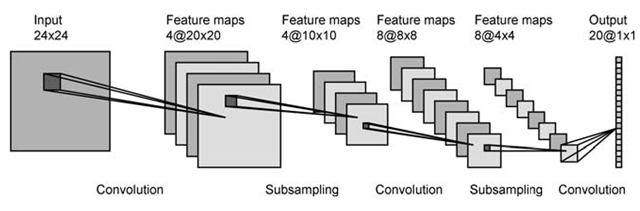
\includegraphics[width=\textwidth]{CNN-Example}
\caption{Example of a CNN network}
\end{figure}

We see here that in the first convolutional layer, the input shape is 24x24 and the kernel size is 5x5, which strides over the input shape to produce 4x(20x20) shapes. Here the number of filters was 4, which is why 4 outputs have been produced. Also, typically the stride size is 1. In this 24x24 input, with a 5x5 filter we can have $(24-5+1)$ possible positions of the filter in one direction. 

\textbf{Subsampling / Pooling:}\\
Subsampling is essentially taking the average across a group of cells to produce a smaller shape. This therefore produces the same number of 'feature maps' but smaller in size. 

\textbf{Fully Connected Layers:}\\
Fully Connected Layers (FCs) take all the feature maps from a convolutional layer and stack them all together in a traditional neural network in which every node is connected to every other node (fully connected). This then allows the network to learn the relationships between small parts of the image (or input in general) on a fine grained level. 


\section{Generative Adversarial Networks}
GAN is a framework proposed by Ian Goodfellow, Yoshua Bengio and others in 2014. The idea is that we have two networks: a generator and a discriminator. The generator network tries to produce,  from random noise,  data in the form of the training data we want. This could be an image, in the common use-case, or in this one, a fraudulent transaction vector. The discriminator, takes in real-life data (from the training set) and also the generated data from the generator network. The discriminator tries to determine whether the current input is real or generated. Effectively these two networks play a game with each other: the generator tries to fool the discriminator whilst the discriminator tries to catch out the generator. This continues until each network doesn't get any better and the GAN stabilises. Figure 2.1 represents an overview of a GAN network.

\begin{figure}[H]

\centering
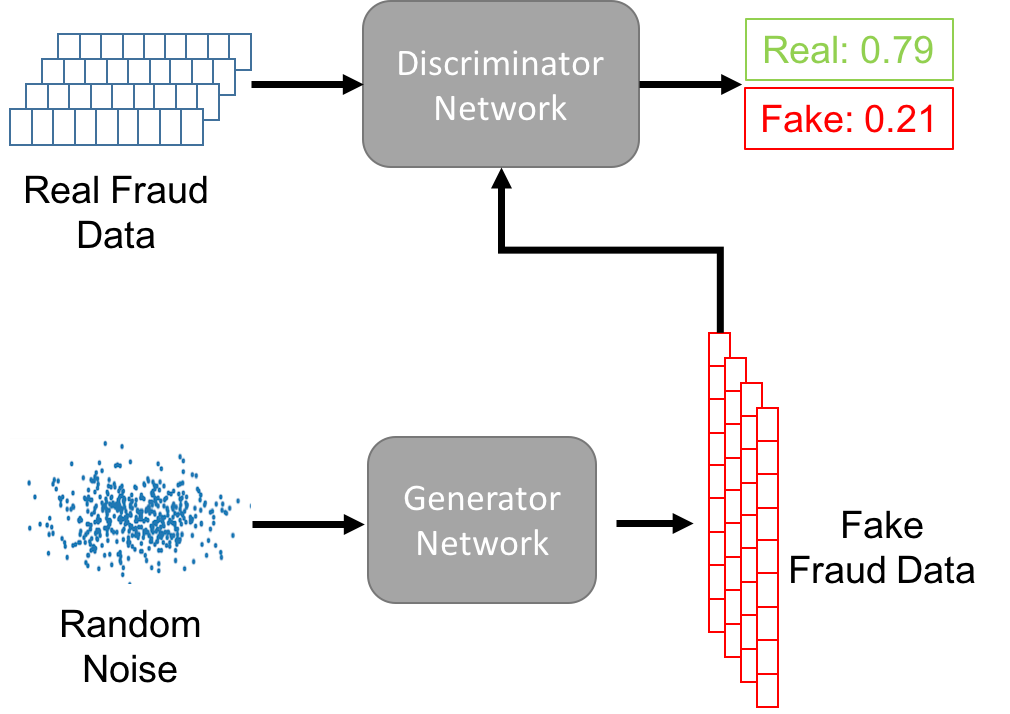
\includegraphics[width=\textwidth]{GAN-Overview}
\caption{Overview of a GAN network}
\end{figure}

Mathematically, we can define the following quantities:

$$X_{x\sim p_\text{data}(x)} = \text{Sample from distribution of real data} $$
$$Z_{z\sim p_\text{z}(x)} = \text{Sample from distribution of generated data} $$
$$G(z) = \text{Generator Network}$$
$$D(x) = \text{Discriminator Network}$$
The process of training for a GAN is like a min-max game between the two networks, and can thus be represented by the following value cost function:
$$\min _ { G } \max _ { D } V ( D ,G )$$
where 
$$V ( D ,G ) = \mathbb { E } _ { x \sim p _ { d a t a } ( x ) } [ \log D ( x ) ] + \mathbb { E } _ { z \sim p _ { z } ( z ) }[ \log ( 1- D ( G ( z ) ) ] $$
The first term in this equation represents the quantity of the real-distributed data passed through the discriminator network. The discriminator tries to maximise this such that $D(x)\rightarrow 1$. The second term represents generated data passed through the discriminator. The generator tries to minimise such that $D(G(z))\rightarrow 1$ (i.e the discriminator is fooled by the generated sample).

The steps for training a GAN can be outlined as followed:
\begin{enumerate}[Step 1:]
  \item 
  \begin{enumerate}
  \item Take a batch of real data and train discriminator to correctly predict them as real
  \item Take a batch of generated data and train discriminator to correctly predict them as fake
\end{enumerate}
  
  \item Freeze the training of the discriminator network
  \item Generate a batch of fake data and use the frozen discriminator to train the generator
  \item Repeat the above for n epochs until neither network makes any further improvments
\end{enumerate}

In summary, we alternate between training of the discriminator to correctly determine real or fake data and training the generator on fooling the discriminator. The reason for freezing the weights of the discriminator while we train the generator is exactly so that we don't alter the weights during this process and the generator can use the current state of the discriminator to become better.

\section{Machine Learning Evaluation Practices}
Here I describe some of the main machine learning evaluation concepts that I had to have a clear idea of, prior to implementation of this project. 

\subsection{Train and Test Splits}
Let's say we have \textbf{\textit{m}} examples $ \mathbf { x } _ { 1} ,\mathbf { x } _ { 2} ,\dots ,\mathbf { x } _ { m }$ each in $\mathbb { R } ^ { n }$. In a supervised learning problem, we also have \textbf{\textit{m}} labels $\left\{ y _ { 1} ,y _ { 2} ,\dots ,y _ { m } \right\}$ in a set \textbf{\textit{Y}}.\\
In machine learning we wish to find a hypothesis $h : \mathbb { R } ^ { n } \rightarrow Y$ that is defined by a vector of weights \textbf{\textit{w}}. It is then common to write $h _ { w } ( x )$.\\

We define a training set as $\mathbf{s} = [(\mathbf { x } _ { 1}, \mathbf { y } _ { 1}),(\mathbf { x } _ { 2}, \mathbf { y } _ { 2}),\dots,(\mathbf { x } _ { m}, \mathbf { y } _ { m})]$.
 
When training a model, to try and achieve our $h _ { w } ( x )$, we use data from the training set. When we train a model, it will often report some metrics or loss function to reflect how the performance increased during the training process. 

The problem with this however is that our model may not perform well on \textbf{unseen} data. In other words, it might not \textbf{generalise} well. To overcome this, it is good practise to preserve a testing portion of the data, called the test set, that is not used in the training process. The test set is then used to evaluate how the model performs after training. 

\begin{figure}[H]

\centering
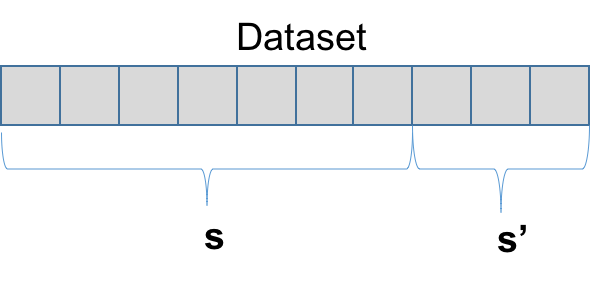
\includegraphics[scale=0.8]{train-test-split}
\caption{A 70:30 train test split of data.}
\end{figure}

\subsection{Cross-validation}

Cross-validation takes this a step further. The hypothesis of our model may in fact generalise and perform better on some portions of the data over others and thus performing just one split, may not give the most confident results. Also, when performing these train-test splits, the element of randomness in the split can work against us as even if we average this process say 3 times, it is likely that there is some overlap in the runs and we are not really using the data available to its full capacity. 

\begin{figure}[H]

\centering
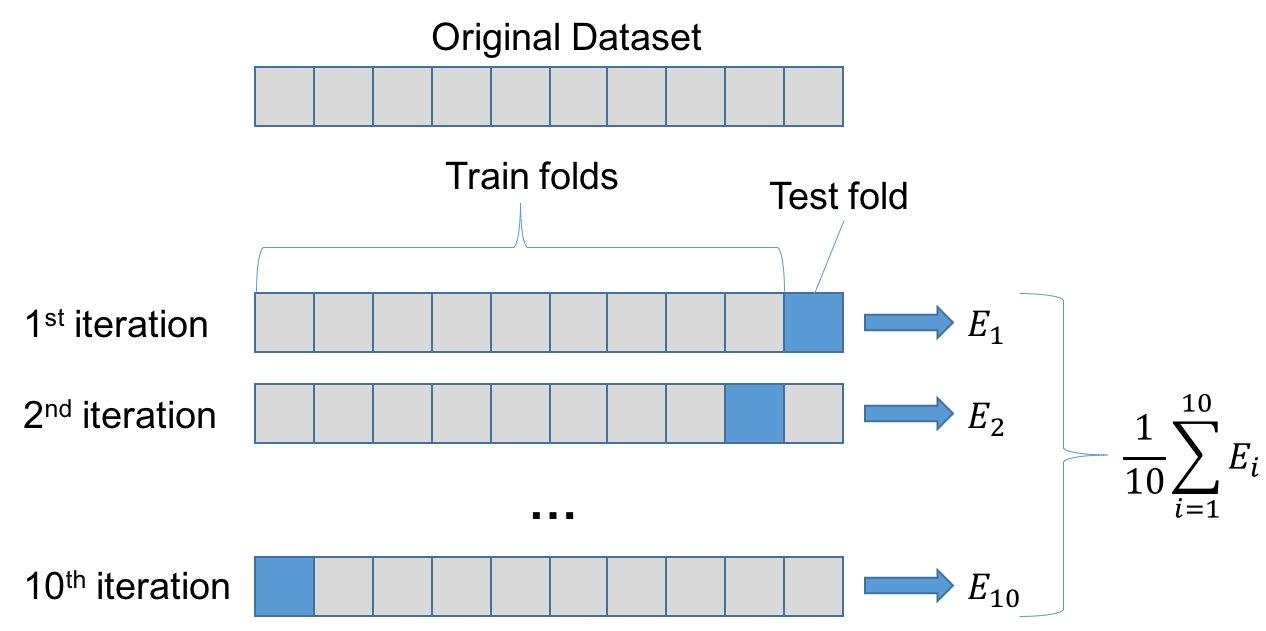
\includegraphics[scale=0.8]{cross-val}
\caption{K-Fold Cross Validation.}
\end{figure}

\subsection{Resampling Methods}

During the baseline work of the project I also experiment with resampling methods. These are ways of balancing the dataset such that the ratio of positive class to negative class is brought to 50:50. I do this to give an example of how these methods affect our results before moving onto the deep learning architectures. 
The three main methods I explored were:

\begin{enumerate}
  \item Undersampling 
  \item Duplicate Oversampling
  \item Synthetic Minority Oversampling Technique (SMOTE)
\end{enumerate}

\subsubsection{Undersampling}
Undersampling is the process of reducing the majority class down to a lower amount, to balance more with the minority class. This can be achieved by randomly removing samples until the ratio is 50:50 or another specified amount. 


\subsubsection{Duplicate Oversampling}
Duplicate Oversampling is a naive method of increasing the amount of the minority data class, to match that of the majority. This works by taking existing minority data points and simply duplicating them.

\subsubsection{SMOTE}
Synthetic Minority Oversampling Technique (SMOTE) is another method of increasing the amount of the minority data but not by duplication as before. SMOTE takes the $k$ nearest neighbours of a data point, randomly selects one of these k neighbours and creates a vector between the two. Then a new, synthetic data point is created some random distance along this vector line, by an amount in the range $[0,1]$.

\subsubsection{Cross-validating Correctly}
When employing oversampling techniques, this completely affects the way we handle cross-validation. It no longer is valid to simple oversample the dataset and then perform cross-validation. The reason for this is the potential of overfitting. Figure~\ref{fig:oversample-before} shows what can happen in this situation. 

\begin{figure}[H]
\centering
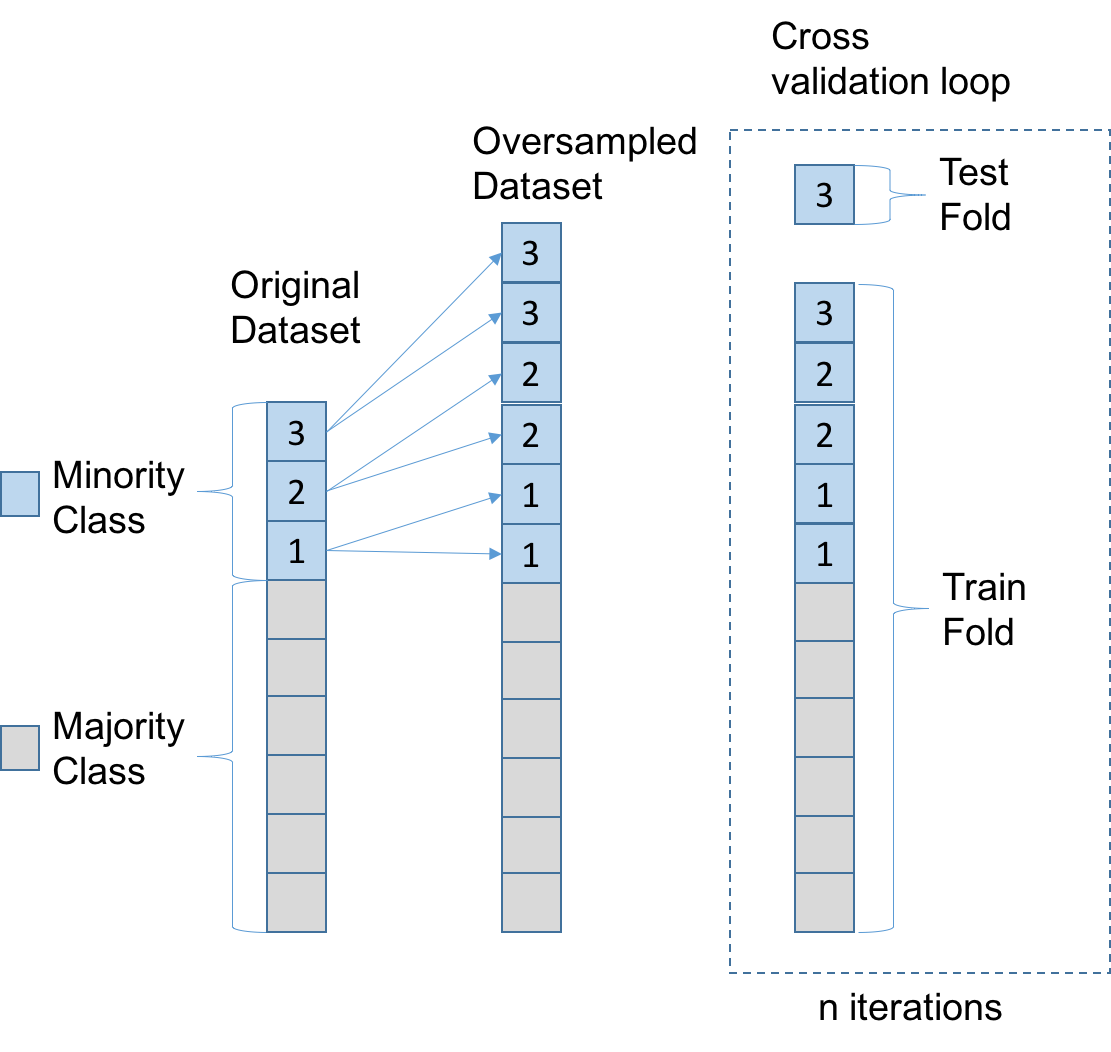
\includegraphics[scale=0.8]{oversample-before}
\caption{Oversampling OUTSIDE the cross-val loop.}
\label{fig:oversample-before}
\end{figure}

Inside the cross-validation loop, the current train-test folds split means that some of the oversampled minority class (node 3) that was portioned into the test set is also in the training set. This means that our model would have seen this data during the training process and will therefore have a bias during the testing and evaluation phase as it already knows how to classify this data. 

It is therefore crucial that this is adapted such that any oversampling occurs inside the cross-validation loop, and not before/outside it. Figure~\ref{fig:oversample-after-1} and Figure~\ref{fig:oversample-after-2} represent the correct way to handle this, for $n=1$ and $n=2$ respectively. For every iteration of the loop, we split the data into train-test first and then oversample the training data fold only. This preserves the testing fold, keeping a portion of the original dataset untouched, for evaluation. This is a lot more effective in testing the generalisability of a model.

\begin{figure}[H]
\centering
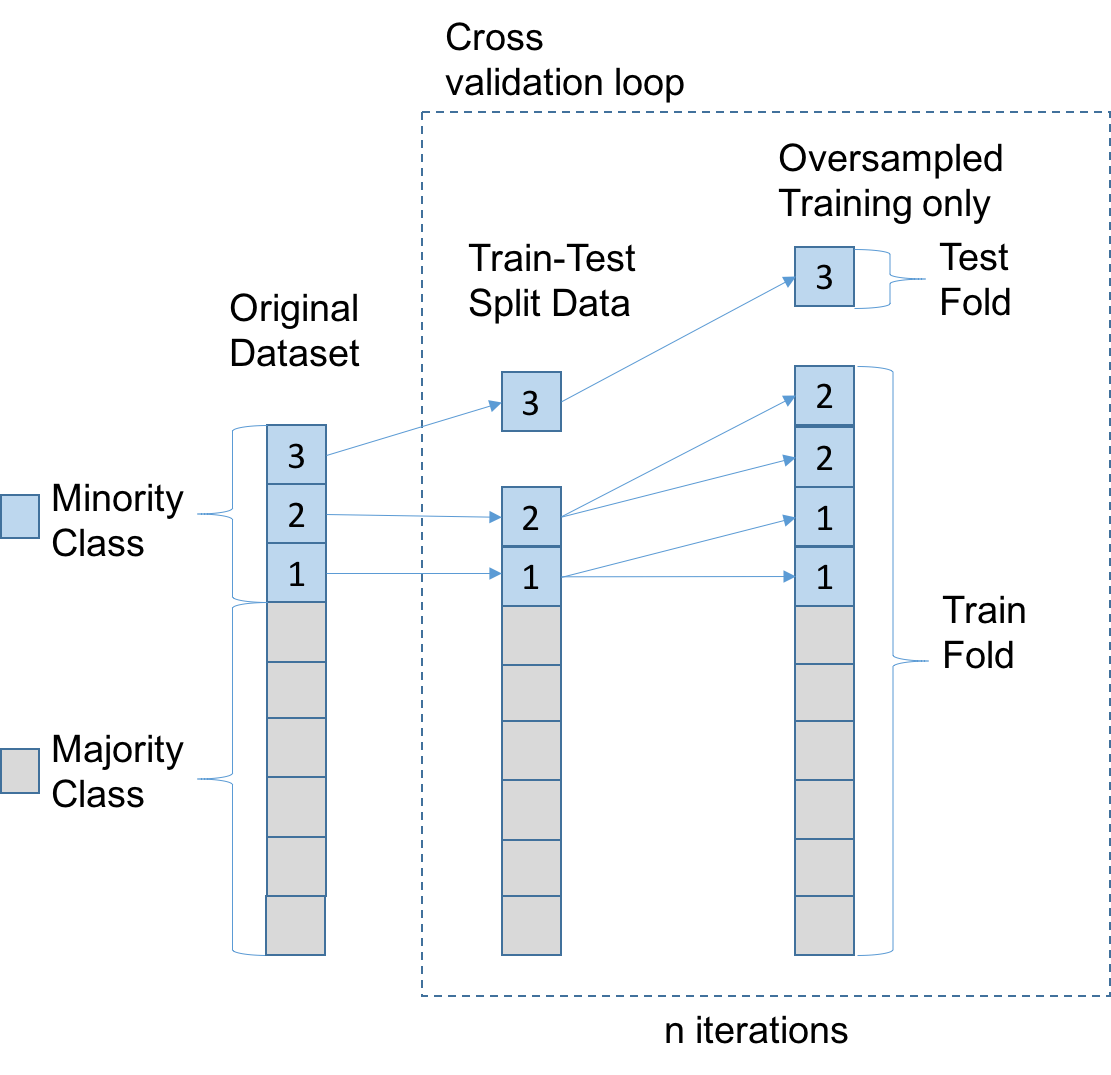
\includegraphics[scale=0.6]{oversample-after-1}
\caption{Oversampling INSIDE the cross-val loop [n=1].}
\label{fig:oversample-after-1}

\centering
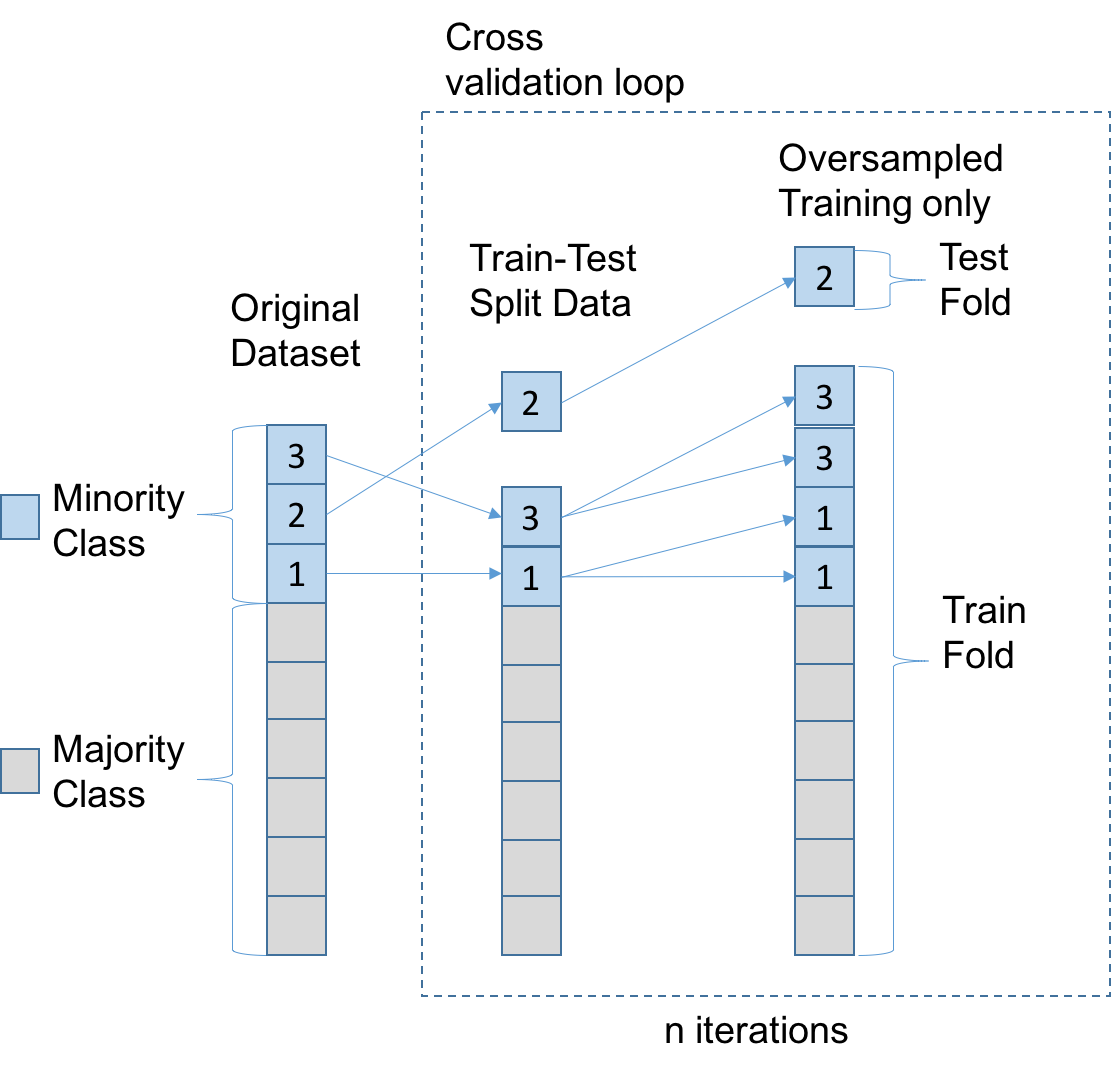
\includegraphics[scale=0.6]{oversample-after-2}
\caption{Oversampling INSIDE the cross-val loop [n=2].}
\label{fig:oversample-after-2}
\end{figure}

% Implementation
\chapter{Implementation}
\section{Models Overview}

\begin{figure}[H]
\centering
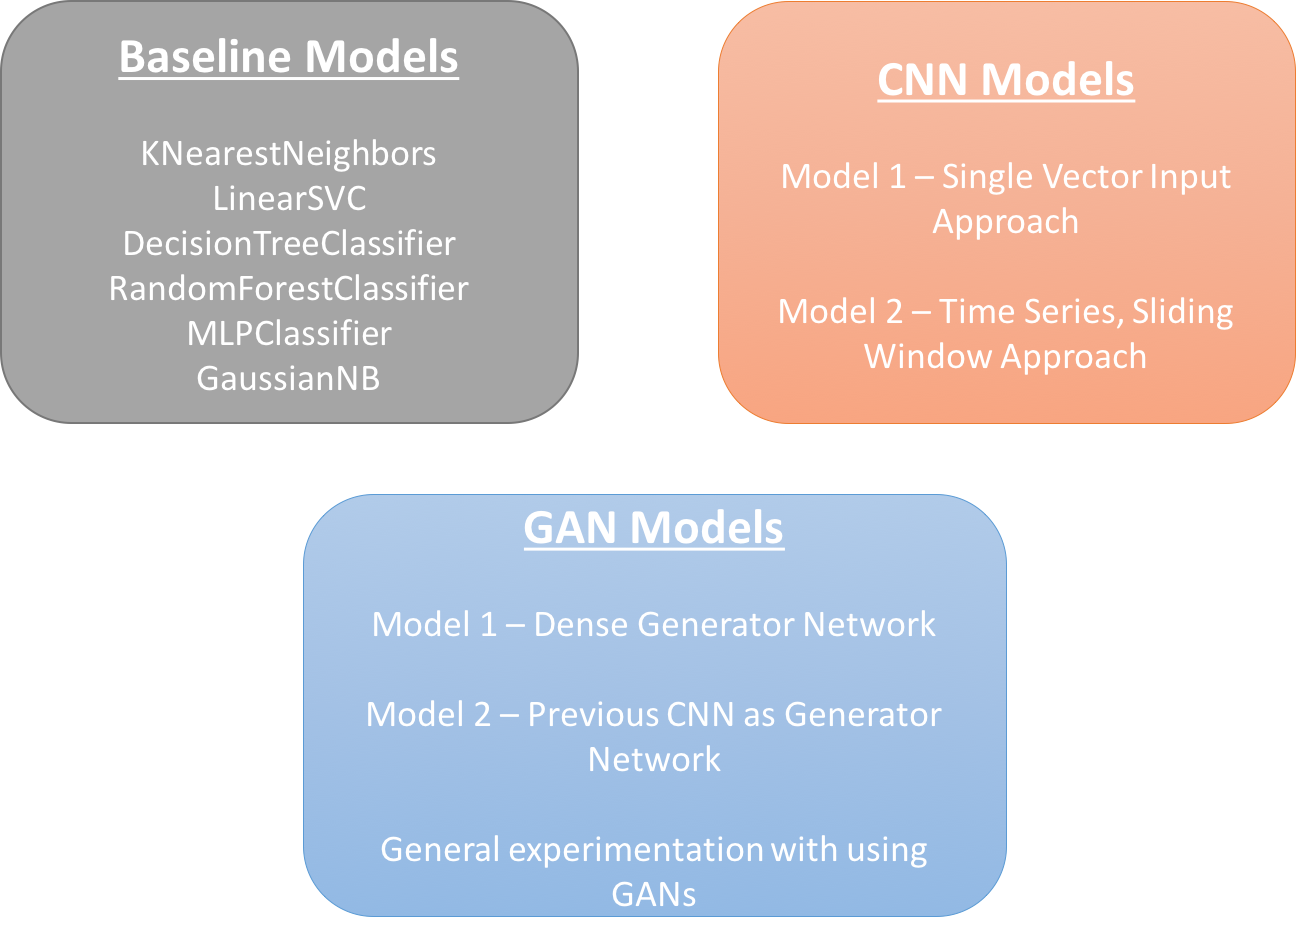
\includegraphics[scale=0.8]{models_overview}
\caption{Overview of models experimented with.}
\label{fig:models_overview}
\end{figure}

\section{Baseline Models}
\subsection{Data Preparation}

\textbf{Feature Scaling}\\

Standardisation involves rescaling the features such that they have the properties of a standard normal distribution with a mean of zero and a standard deviation of one. This is very important in machine learning when features can be a lot larger in magnitude than others. For example, if one feature is age and another is salary in USD then these two quantities will be on different ranges and the salary feature may negatively impact classifier algorithms by deeming that feature to be more important and confusing the weights assignment. Scaling solves this problem. 

Therefore one of the first steps was to scale the features, which I did using StandardScaler from SKLearn. 

\textbf{Feature Engineering}\\

In many machine learning and data science applications, feature engineering is something used to add additional features based on calculations and domain knowledge of the data. In this case, though, as the data is already post-PCA and the time-series span of the transactions is only over 2 days. I decided not to do any feature engineering and to just employ algorithms on the original dataset features.

\textbf{Sanity Checks}\\

Also, I checked the data to see if any values were missing, or null. This was to ensure that the data was clean to be passed through machine learning networks. There were no missing data in this case.

\subsection{Cross Validation Function}

Defining my own cross-validation function early on was a crucial step in this project. As explained briefly in the preparation chapter, the way in which cross-validation is performed is very important to ensure no overfitting occurs and that the results are as confident as they can be. As far as implementation is concerned, It was not enough to use the built in SKLearn cross-val function as it did not provide enough granularity in it's output. I wanted very specific metrics and not to mention, I needed to resample data in the correct place which meant I needed to define my own function, based on the standard library which uses Stratified KFold. This essentially means that the splitting of the data in each fold of the KFold procedure, contains at least some portion of the underrepresented class. This is important as it would be very common that some folds don't contain any of the minority class. 

The function uses a utility function from SKLearn, \textbf{precision\_recall\_f1}, which simply reports the precision, recall and f1-score for predicted values. You give it a set of predicted values and the set of true values and it calculates the metrics. I use this inside my function to report the metrics we are interested in, something I could not do originally. 

\begin{algorithm}[H]
\caption{Cross-Validation function }\label{cross-val}
\begin{algorithmic}[1]
\Procedure{custom-cross-val}{$X, Y, CLF, N$}

   \State $skfolds\gets \textbf{StratifiedKFold}(n\_splits = N)$\\
   
   \State $precisions\gets []$
   \State $recalls\gets []$
   \State $f1scores\gets []$
   \State $elapsedtimes\gets []$\\
   
   \For{\texttt{train\_indices, test\_indices in skfolds.split(X,Y)}}
        \State
         \texttt{\State $X\_train\_folds\gets X[train\_indices]$}
        \texttt{ \State $Y\_train\_folds\gets Y[train\_indices]$}
        \texttt{ \State $X\_test\_folds\gets X[test\_indices]$}
         \texttt{\State $Y\_test\_folds\gets Y[test\_indices]$}
         
         \texttt{\State $X\_res, Y\_res \gets \textbf{Resample}(X\_train\_folds,Y\_train\_folds)$}
         
          \texttt{\State $ start \gets current time$} 
          \texttt{ \State \textbf{CLF.fit}($X\_res, Y\_res$)} 
          \texttt{\State $ end \gets current time$} 
          \texttt{\State $ elapsed \gets end - start$} 
          \texttt{\State elapsedtimes.append(elapsed)} 
           \texttt{\State $y\_pred \gets \textbf{CLF.predict}(X\_test\_folds)$} 
          \texttt{\State $stats \gets \textbf{precision\_recall\_f1}(y\_pred, Y\_test\_folds )$} 
          
          \texttt{\State precisions.append(stats[0])}
          \texttt{\State recalls.append(stats[1])}  
          \texttt{\State f1scores.append(stats[2])} 
   \EndFor
   
   \State \textbf{return} [ mean(precisions), mean(recalls), mean(f1scores), mean(elapsedtimes) ]
   
\EndProcedure
\end{algorithmic}
\end{algorithm}

This is something I could then use for varying \textbf{Resample} methods. 

\subsection{Cross Validation the Wrong Way}

\textbf{Test\_Train\_Split vs Custom cross\_val\_score using KFold}\\
This concerns the underlying approach for the cross validation loop. SKLearn's test\_train\_split function splits the data into train and test portions. We can then oversample our training data, fit the model and make predictions using the test set.
One approach that perhaps would be a logical one, would be to simply do this multiple times and average the results.
This approach, however, will give better results than expected (which I showed in my experiments, results outlined in the evaluation chapter). The reason for this is due to the nature of test\_train\_split and it's randomness.

Test\_train\_split allows you to randomly split your data, by giving a parameter that specifies the ratio. However as the split is random, it is likely that there will be overlap in the CV iterations as to which data points are put in the test set. In other words, values selected during one iteration, could be selected again during another iteration.
The consequences of this means that the model may not be exposed to particular portions of the data whereby it does not generalise well and we are not capturing that in our results. Also, It is not making maximal use of the data we have.

I ran my classifiers using this approach, too, as a means of comparison of what can go wrong and give invalid results, if you're not careful. The correct way, the way which was detailed above, is using KFold cross validation to split the data during a loop and doing any customisations or resampling inside this loop.

\subsection{Resampling functions}
To implement resampling functions I made use of the \textbf{imbalanced-learn}\cite{JMLR:v18:16-365} library. This is an API that focused on methods for unbalanced datasets, including oversampling and SMOTE techniques. They have written functions that do exactly what I needed so I made use of their work in this small part of my project. 

I created simple functions in the form of:\\
\textbf{Input: X data, Y data}\\
\textbf{Output: X-res, Y-res}\\
Where X-res and Y-res are the resampled X and Y data. 

\textbf{Duplicate Oversampling}\\
For random, duplicate Oversampling I used their \textbf{imblearn.over\_sampling.RandomOverSampler.} This does as I described in the preparation chapter. Randomly selects a datapoint and duplicates it, or in other words 'selecting random data points, with replacement'.

\textbf{SMOTE}\\
For SMOTE, I used their \textbf{imblearn.over\_sampling.SMOTE}. The default parameter of k\_neighbors was used, which is a value of 5, which was fine for this use. 

\subsection{Collecting Results for All Classifiers}
By using the carefully constructed cross-validation algorithms defined above for the various resampling methods, I constructed a general algorithm to loop through the classifiers i'm interested in and running cross-validation for each of them, for each resampling method and collating results in a Python DataFrame log. 

The algorithm outline can be viewed as follows:

\begin{algorithm}[H]
\caption{All Classifiers Run }\label{all-classifiers}
\begin{algorithmic}[1]
\Procedure{all-classifiers-run}{}
        \State
         \texttt{\State $classifiers \gets [KNeighborsClassifier, LinearSVC, DecisionTreeClassifier,$\\ $RandomForestClassifier, MLPClassifier, GaussianNB]$}
          \texttt{\State $columns \gets ["precision", "recall", "f1", "auc", "training-time"]$}
         \texttt{\State $log\_original \gets DataFrame(columns = columns)$}
         \texttt{\State $log\_under \gets DataFrame(columns = columns)$}
         \texttt{\State $log\_over \gets DataFrame(columns = columns)$}
         \texttt{\State $log\_smote \gets DataFrame(columns = columns)$}
         
   	\For{\texttt{clf in classifiers}}

            	\State {$log\_entry\_original\gets  \textbf{cross\_val\_original}(data, clf, 3) $}
            	\State $log\_entry\_under\gets  \textbf{ cross\_val\_under}(data, clf, 3) $
            	\State $log\_entry\_over \gets \textbf{cross\_val\_over}(data, clf, 3) $
            	\State $log\_entry\_smote \gets \textbf{cross\_val\_smote}(data, clf, 3) $
            	\State $log\_original \gets \textbf{log\_original.append}(log\_entry\_original $
            %	\State
   	\EndFor
   
   \State \textbf{return} [ mean(precisions), mean(recalls), mean(f1scores), mean(elapsedtimes) ]
   
\EndProcedure
\end{algorithmic}
\end{algorithm}

I used Python DataFrames as they were a convenient method of storing the results and meant I could construct tables of results in a very organised way. Also, DataFrames have nice methods for plotting data and saving the results to disk. 


\section{Convolutional Neural Network Models}

\subsection{Overview}
In this section, I describe the work I completed in constructing the CNN models and retrieving results using these models. I experimented with two main approaches that were briefly designed and outlined in the initial stages of the project. The main goal here is to see if it is suitable and indeed effective to use these types of deep learning models on time series data, specifically with the credit card fraud data. Prior to implementing these models, I had to do thorough reading of how CNNs work (detailed briefly in the preparation chapter).


\subsection{CNN Version 1}

\subsubsection{Version 1-1}
In the first proposed approach for my CNN models, the network bridges from our baseline models by keeping single vector data as inputs. In other words, the input to the first CNN is still a 30 x 1 transaction vector. I then introduce convolutional aspects to the network and aim to construct a model appropriately based on the output of each layer. 

Figure~\ref{fig:cnnv1} shows the outline of basic CNNv1 network.

\begin{figure}[H]
\centering
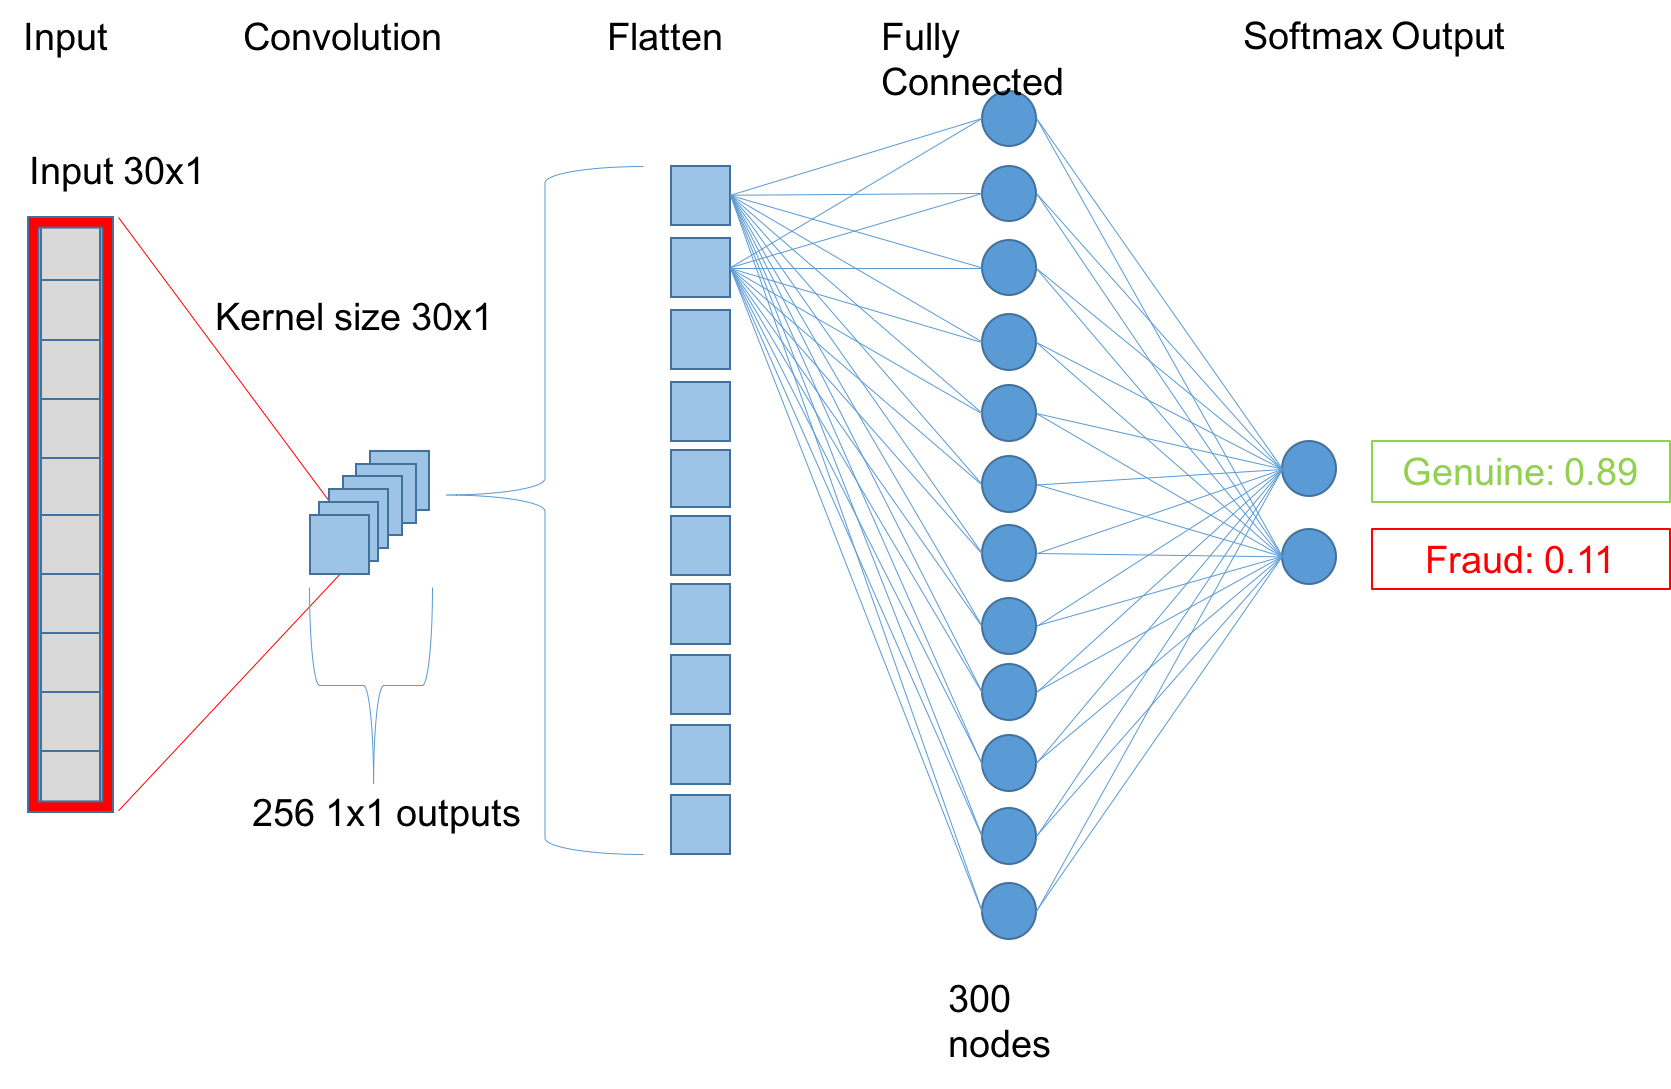
\includegraphics[scale=0.6]{cnnv1}
\caption{Overview of CNN Model 1.}
\label{fig:cnnv1}
\end{figure}

The input layer takes a transactional vector. Then, a convolutional layer performs convolutions on the input data, using 30x1 kernels, of which there are 256, differently initialised. This creates 256 1x1 outputs. By flattening these outputs, I then introduce a fully connected layer, which essentially means that every node is connected to every other node, between the flattened layer and the subsequent dense layer of which I used 300 nodes. Then there is a softmax output layer which takes the weighted sum of the fully connected layer and also has an activation, as with usual neural network architectures and gives us our predictions, corresponding to Fraud or Genuine.

\subsubsection{Version 1-2}
In an attempt to take this model a little further, I tried a variation whereby I added an extra convolutional layer and also an extra dense layer in the fully connected section. This was to give an indication of effect of additional layers would have.

The results of this version was also reported and compared with Version 1-1. 

Listing~\ref{lst:cnnv1-1-createmodel} is a code snippet that shows the short function that creates CNNv1-1. 

\lstinputlisting[language=Python, caption=CNNv1-1 create\_model function., label={lst:cnnv1-1-createmodel}]{code-snippets/cnnv1-snippet-1.py}

Listing~\ref{lst:cnnv1-2-createmodel} is a code snippet that shows the short function that creates CNNv1-2. 

\lstinputlisting[language=Python, caption=CNNv1-2 create\_model function., label={lst:cnnv1-2-createmodel}]{code-snippets/cnnv1-snippet-2.py}



\subsubsection{ReLU Activations}

On each hidden layer, I use the Rectified Linear Unit (ReLU). In modern deep learning applications, the use of the ReLU activation is very popular and there are valid reasons for this, one perhaps most prominent is mitigating the vanishing gradient problem. 

The ReLU function is defined mathematically as:
$$f ( x ) = x ^ { + } = \max ( 0,x )$$

The Sigmoid Activation is defined as:
$$S ( t ) = \frac { 1} { 1+ e ^ { - t } }$$

The gradient of sigmoid is:

$$S ^ { \prime } ( t ) = S ( t ) ( 1.0- S ( t ) )$$

\textbf{Vanishing Gradient Problem}
During gradient based learning methods, a weight update is back propagated through a network. We see that the gradient of a sigmoid activation will be close to zero if the output is close to the tail ends of 0 or 1 (saturated neurons). This is a problem when there are multiple layers to the network as we multiply near-zero quantities every time and hence we have a 'vanishing gradient'. This means that even large changes, will attenuate through the network and result in affecting the output less. The hyperbolic tangent function activation also has this saturation problem. 

The ReLU activation however, has a constant gradient. This means there is no attenuation in the back propagated signal and actually training is faster. The mathematical calculations are easier too, as the ReLU does not use exponentials. In the ImageNet\cite{krizhevsky2012imagenet} paper by Krizhevsky et al, they show the effect of using ReLU with respect to speed of training. 

\subsection{CNN Version 2}

\subsubsection{Overview}

Version 2 aims to explore more the idea of arranging the transactions temporally and trying to use the image metaphor, to unravel relationships in the data. In this setup, a bit more preprocessing is needed in order to suit the network. The model itself takes an input batch of 100 vectors, so we have a 100 x 30 block. Then here our kernel (or filter) is 5 x 30 block which slides down the temporally ordered block and convolves with the features, to give the output. 

Doing some maths here, a window of height 5, can be positioned in 96 unique positions over the batch. Again, the model uses a number of different filters which are initialised. Figure~\ref{fig:cnnv2-1} shows this process, using 32 different kernels. This gives an output of 96 (from the convolution) x 32 (the number of different kernels).

\begin{figure}[H]
\centering
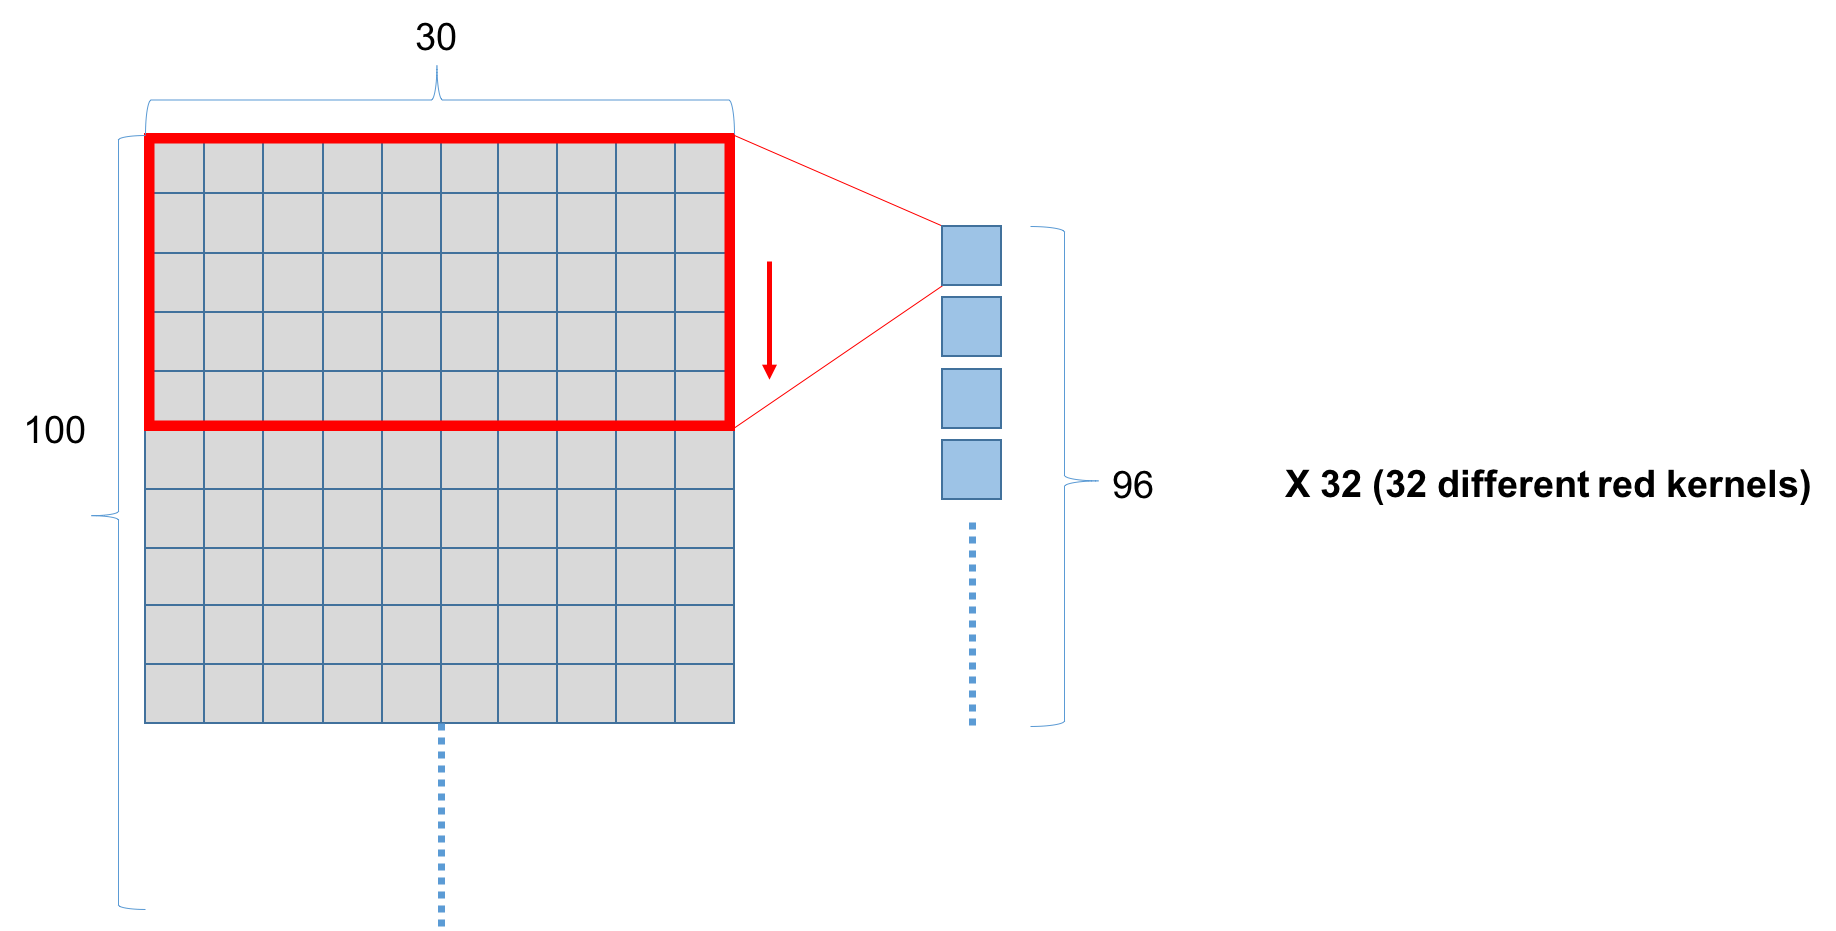
\includegraphics[scale=0.5]{cnnv2-1}
\caption{Overview of CNN Model 2 - Part 1.}
\label{fig:cnnv2-1}
\end{figure}


Figure~\ref{fig:cnnv2-2} then shows the remainder of the model. The output from the convolutions are flattened and hooked up to a fully connected layer. Then the softmax output layer, as before, to output our classification probabilities. 

\begin{figure}[H]
\centering
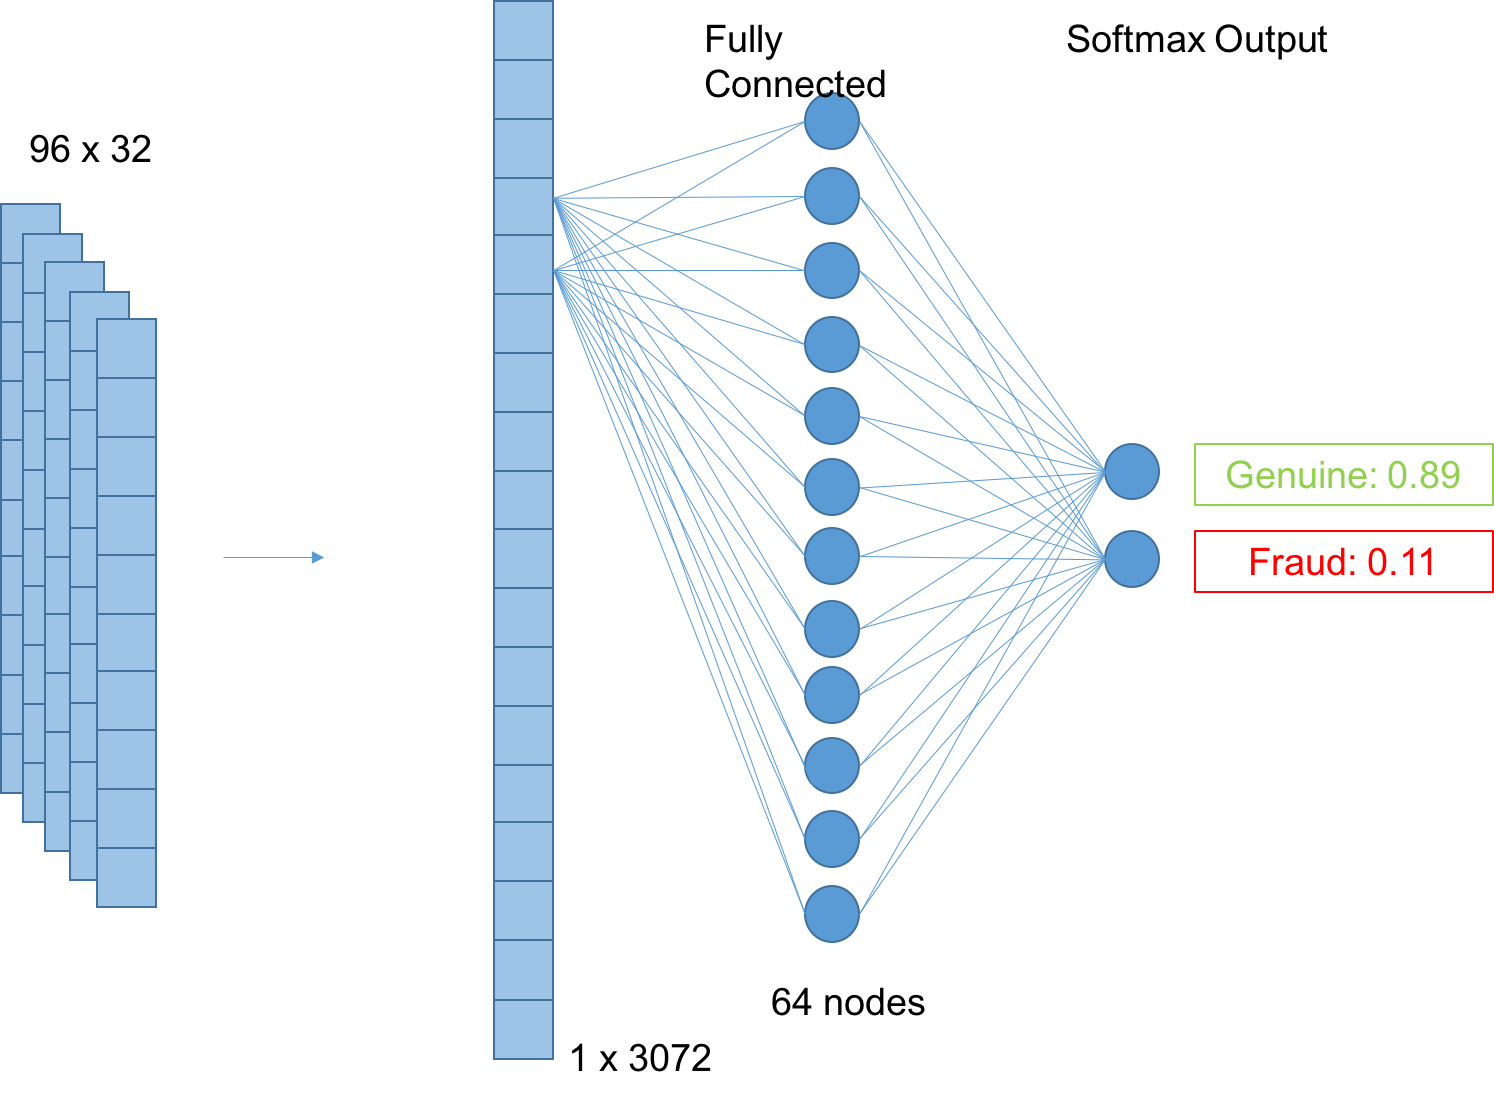
\includegraphics[scale=0.6]{cnnv2-2}
\caption{Overview of CNN Model 2 - Part 2.}
\label{fig:cnnv2-2}
\end{figure}

\subsubsection{Preprocessing}

Due to the nature of this network, a lot more care has to go into preprocessing the data so that we can pass it through the model. One important thing is to batch together the dataset into chunks of size 100 (in this case), as this is the input of the model. So if the original size of the training data is (199365, 30), then we want to transform this to (1994, 100, 30). However, if the length of the training set is not a whole multiple of 100 then there will be a problem with the final batch. In order to fix this, the final batch is padded with zeros. 

Listing~\ref{lst:cnnv2-batchreshape} outlines a function that packs up this transformation into a function that can be reused for varying values of this hyper-parameter.
\lstinputlisting[language=Python, caption=CNNv2 batch reshape function., label={lst:cnnv2-batchreshape}]{code-snippets/cnnv2-batch-reshape.py}

\subsubsection{Time-Series Cross-Validation}

Due to the fact that this CNN model specifically exploits the temporal ordering of the transactions, the usual method of cross-validating becomes insufficient. This is because during the usual, KFold procedure, the data will be split randomly and of course this will violate temporal ordering. In general, cross-validating for predictive modelling like this is tricky, but there are a ways of doing it. I outline one here in my implementation. 

The approach is to split the data as usual (perhaps a 70:30 split), but keeping the temporal ordering such that every transaction after the cutoff point (i.e in the testing set) has a transaction with time $T > T_{n} $, where $T_{n}$ is the last transaction of the training set. When transactions are ordered by time, in the real world we often predict only the next one or two time steps (think of stock market fluctuations). We can use this therefore to average results across the size of the testing set, progressively predicting less test data. 

This can be visualised as follows:

$$ [1] [2] [3] [4]  --- [5] [6] [7] , \hspace{5mm}  n=1$$
$$ [1] [2] [3] [4] [5] --- [6] [7] ,\hspace{5mm}  n=2$$
$$ [1] [2] [3] [4] [5] [6] --- [7] ,\hspace{5mm}  n=3$$

The implementation of this is through wrapping the model creation into it's own function, like previously, taking parameters to make the batch-size and window-height dynamic. Inside the cross-validation function itself, the preprocessing, model creation and model predictions are all wrapped up together. There is also another auxiliary function that generates the time-series split of the data by ordering it and splitting it at a specified ratio, given to the function as a parameter. Inside the cross-validation this function is called with decreasing value, to return a progressively larger training set and smaller test set with every iteration. 

\section{Generative Adversarial Network Models}

\subsection{Overview}
As described in the preparation chapter, GANs are essentially two networks that play a game with each other, each trying to reduce their own loss function. 

The three major components of a GAN are the generator network, the discriminator network and the combined network training process. Below, I outline the steps needed in the adversarial training stage of the GAN, as well as various utilities that were import to the setup and running of the models. 

Then this section outlines the three major variations in which I experimented; two variations on the generator network and then an attempt at incorporating a semi-supervised learning approach to treat the GAN as a classifier. This came about due to the fact that GANs in their common use case, display how the networks perform with regard to their loss functions and also can display the intermediate generations (like in the classic MNIST dataset) to visually inspect how the GAN is performing. Seeing as the data I am working with, is inherently used in classification problems, it is of interest to experiment with using the GAN as so. However, simply investigating how the generator performs at constructing fraud-like data is also very interesting, this could have potential of helping the domain create more data on which to train with. 

Below, listing~\ref{lst:gan-classdefinition} shows the abstract definition of the GAN class, in which I wrapped up all of the main functions of the model. This definition shows the prominent functions with short descriptions. 
\lstinputlisting[language=Python, caption= GAN Class Definition., label={lst:gan-classdefinition}]{code-snippets/GAN-classdefinition.py}

\subsection{Adversarial Training}

The training procedure of the GAN is a crucial component. Unlike other models in Keras, a GAN is not nicely wrapped up in one library function and so we have to connect up networks ourselves and implement the training process from scratch. This is what I did in the GAN class. The training process must do a number of things, which I outline below in a high-level pseudo-code algorithm:

\begin{algorithm}[H]
\caption{Adversarial Training }\label{gan-train}
\begin{algorithmic}[1]
\Procedure{Gan-Train}{$self, epochs, batch\_size=128, save\_interval=200$}
	
        \State \textbf{Get X and Y train data}
        \State \textbf{Reshape training data into tensors} 
        \State 
         
   	\For{\texttt{epoch in epochs}}
		\State
		\Comment Discriminator Training 
		\State \textbf{Take a random half batch of training data}
		\State \textbf{Generate, using the generator, a half batch of fake data}\\
		\State \textbf{Set discriminator.trainable = True}\\
		\State \textbf{Create half batch number of labels for the real and fake data}
		\State \textbf{Format labels into categorical shape}
		\State \textbf{Train discriminator separately on real and fake data}
		\State \textbf{Set discriminator.trainable = False}\\
		\State
		\Comment Generator Training 
		\State \textbf{Create random noise} 
		\State \textbf{Create associated positive labels for the random noise}
		\State \textbf{Train the Combined model using this noise and labels}\\
		\State \textbf{Save and Append losses of both networks }
		\State
		\Comment Save Intervals
		\If{epoch \textbf{mod}  save\_interval == 0}
			\State \textbf{Save current generated output}
		\EndIf
   	\EndFor
   
\EndProcedure
\end{algorithmic}
\end{algorithm}

The Adversarial Training algorithm shown is a very high level outline of the procedure. Some lines in particular contain a lot under the hood:

\textbf{Line 3: Reshape training data into tensors}. This line takes the training data and expands the dimensions in order to satisfy the 3D tensor requirement of the models. This is due to TensorFlow being the underlying engine. 

\textbf{Line 13: Format labels into categorical shape}. Because I used categorical cross-entropy loss in the combined GAN model, the labels of the data needs to be in a binary matrix representation. Targets are in categorical format (e.g. if you have 2 classes, the target for each sample should be a 2-dimensional vector that is all-zeros except for a 1 at the index corresponding to the class of the sample).

\textbf{Line 20: Train the Combined model using this noise and labels}. As outlined in the subsections below, in order to train the generator, we need the discriminator too and thus this is a combined model. The model must be carefully defined so that the loss of the combined model incorporates the loss of the generator. Essentially the networks are stacked together. This is also why in \textbf{Line 15}, we set the discriminator to untrainable (i.e frozen) so that the current state of the network can be used when training the generator in order to allow it to improve. 

\textbf{Line 22: Save and Append losses of both networks}. This line covers the work of saving the loss of each network with every epoch, in order to do things like plotting the loss curves for visual evaluation.

\textbf{Line 25: Save current generated output}. When the save interval is reached, a utility function is called that I implemented to do a number of things. One of which was to use the current state of the generator to take some random noise and generate an output. This is so that we can visualise what the current output looks like at this epoch. This function also includes the various plotting utilities that builds up the final figure which shows generated output for regular training intervals. 

Notice also, how we train the discriminator on real and fake data separately, to give a stable and clear separation of the data.

\subsection{GAN Version 1 - Dense Generator}

In the first GAN version I focus on creating the generator network from scratch, instead of importing one of the previous CNN models. The dense generator network takes in random noise as input, has a series of hidden dense layers and includes regularisation layers such as Leaky ReLU activations and Batch Normalisation.

An outline of the dense generator network can be viewed as:
\lstinputlisting[language=Python, caption= GAN v1 - Dense Generator., label={lst:ganv1-generator}]{code-snippets/ganv1-generator.py}


\subsubsection{Leaky ReLUs}
I use leaky ReLU to allow gradients to flow backwards through the layer unimpeded. TensorFlow does not provide an operation for leaky ReLUs, However the Keras API has a nice wrapper for adding this as a layer. The alpha parameter is essentially how 'leaky' we want the negative gradient to be and in a lot of cases we just want this to be slight, to avoid it being completely zero and so a value of 0.2 is emplyed here. This is something that is quite common amongst GAN papers, in particular in DCGAN(deep convolutional GAN)\cite{DBLP:journals/corr/RadfordMC15}. One of the main problems Leaky ReLUs solve is the dying ReLU problem, whereby a large gradient flowing through a ReLU node could cause the weights to update in such a way that the neuron will never activate again. It is common on large scale networks that a large proportion is 'dead'. I care about this here in the GAN, as the network is very dense in terms of the amount of epochs we train on the data and so I want to mitigate this problem. 

\textbf{Batch Normalisation} layers aim to increase stability of the networks (which in GANs is something we really care about) by normalising node outputs, just like we do to data in the original preprocessing stages.

\subsubsection{The Adam Optimiser}
The Adam optimiser is one which is often seen as the default to use in modern deep learning applications, due to empirical evidence reported in the original paper\cite{DBLP:journals/corr/KingmaB14} whereby it is stated ``Using large models and datasets, we demonstrate Adam can efficiently solve practical deep learning problems" and showing it's performance over that of other optimiser functions. 

To this end, I used the Adam optimiser as the primary algorithm in my models. Adam is not like classical stochastic gradient descent, whereby a single, constant learning rate is maintained across all weights but instead the method computes individual adaptive learning rates for different parameters.

By altering the learning rate in the Adam optimiser, I was able to see better convergence in my GAN loss graphs. 

\subsubsection{Training Variations}

Given that this is very experimental, I also tried variations of the models in order to see what effect they had on the loss curves and generated outputs. The idea being that these may combat the main problem of one network overpowering the other. I outline some of the variations I tried below.

\begin{itemize}
\item Standard adversarial training: with each epoch, the discriminator and generator are training independantly. 
\item Pre-training the discriminator for 500 epochs and then letting the generator learn for the remainder.
\item Alternating between training the discriminator for 500 epochs and then the generator for 500 epochs.
\item Using SMOTE on the data
\end{itemize}

In addition to these, I adjusted the learning rate of the Adam optimiser. 

\subsection{GAN Version 2 - Previous CNN Generator}

The second GAN model was set up with the aim that the generator network would be convolutional and also, be the same as one of our previous CNN experiments. I used the model from CNNv1. This meant that I had to add some functionality to save the model to disk and load the model into the GAN program, conserving the weights. An extra layer of complexity is that I needed to be able to adapt the layers, the output layer needs to be changed to one in which the output is of the shape we want. To do this, I popped the last layer of the model and constructed a dense and reshape layer to model the generated shape we need (which in this case is a 1 by 30 vector, but in 3D tensor form). Then, using the Keras functional API to wrap layers around each other, I constructed the generator by hooking up the input of the loaded CNN model, with the adapted layers. 



\subsection{Semi-Supervised Learning for Classification}

Semi-Supervised learning\cite{odena2016semi} is an approach in which the output of the discriminator network is altered such that the network splits the real probability into N classes and thus giving us means of classifying with the model. 

A difficulty that lies with trying to use the GAN as a classifier, is in the decision of what to base the generative model on. In the previous models, I was experimenting mainly on how well we can learn and generate fraudulent data and with some parameter tweaking, a stable GAN could be achieved with interesting results. However If we want to classify between Fraud and Genuine as well as Fake and Generated then the network needed to be training on the genuine examples too. 

Some problems that can occur here are fairly logical. If we only train to generate fraud then the network might learn that all fraud-like data is simply fake. On the other hand if we train the generator to generate a transaction in general (i.e both fraud and genuine) then the imbalance in the dataset may have a hard time to pick up fraud. 
I experimented with a few variations to see how classification results compare. 
These variations were: generating fraud only, providing the discriminator with half fraud and half genuine examples from the real data and just trying to generate transactions in general from providing the discriminator with original dataset examples.

One important key factor with GANs is the number of epochs. Letting the training process go on for a longer time could potentially have a great effect on results obtained. This was very much part of the experimentation process. In the case of the GAN variations, this proved to decrease the number of misclassified benign transactions, significantly.

Figure~\ref{fig:gan-ssl} below shows a diagram that outlines the change that the semi-supervised approach has on the output of the discriminator network. Effectively this is a form of multi-task learning; one output is a sigmoid layer that gives us the probability of an example being fake or generated and the other is a softmax output which gives us probabilities of class labels, as discussed. The dynamic of the GAN changes here, the discriminator becoming the predominant network that learns to classify. 

\begin{figure}[H]
\centering
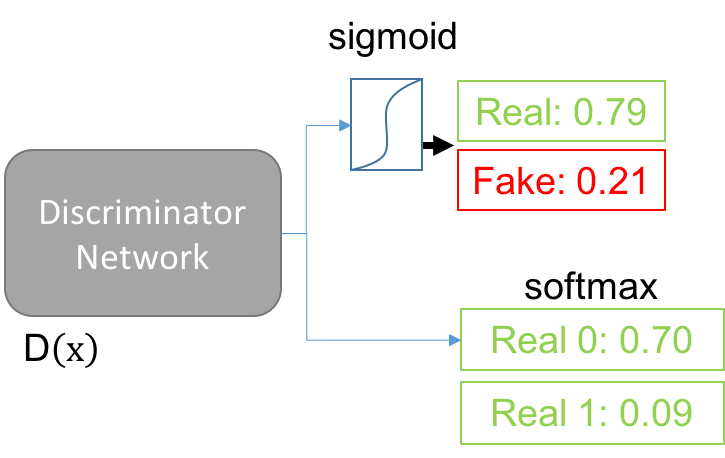
\includegraphics[scale=0.8]{gan-ssl}
\caption{Overview of GAN-SSL discriminator output.}
\label{fig:gan-ssl}
\end{figure}

\subsubsection{Problems with GANs}

\textbf{Mode Collapse}: One problem when training the GAN for a large number of epochs, is a problem called Mode Collapse. This can be visualised in the generated output when the data distributed 'collapses' and suddenly becomes a lot more refined. This is the network learning a certain range and shape of data particularly well and disregarding the rest. In attempt to mitigate this problem you can try adjusting the number of epochs for which you let the network run, to try and best capture the data distribution. 


% Evaluation
\chapter{Evaluation}
\section{Evaluation Methodology}
\subsection{Metrics}
In this project, the metrics that were of interest were not just simply the accuracy, as with many machine learning applications. Accuracy simply measures how many correct classifications are made. This, in the context of credit card fraud, is useless. This is because, even if we classified all fraud as benign, the classifier would still be over 99\% accurate, due to the high imbalance of the fraud/non-fraud classes. In the dataset being used, fraud accounts for only 0.17\% of the total. 

\subsubsection{Precision and Recall}

Therefore we need to look at metrics that tell us more about what we're interested in. Two main measures of interest are \textit{Precision} and \textit{Recall}.

\[
    {Precision} = \frac{T_p}{T_p+F_p} \hspace{5mm} , \hspace{5mm} {Recall} = \frac{T_p}{T_p+F_n} \hspace{1cm}  {T_p} = {True Positive} \hspace{5mm},\hspace{5mm} {F_n} = {False Negative}
\]

Precision is intuitively the ability of the classifier to not misclassify. Recall is intuitively how well to catch fraudulent examples. 

Of course the threshold by which we allow benign transactions to be misclassified as fraud, is a business decision. In the context of a bank, of course the number of fraudulent transactions caught is very important but at the same time we care about precision as this amounts to freezing customers accounts, sending text messages even though they are not subject to fraud, which ultimately costs the bank time and money and potentially customers.

\subsubsection{F1-Score}

F1-score is the harmonic mean of both precision and recall. In general, F-measure can be defined as:
$$F = \frac { 1} { \alpha \frac { 1} { P } + ( 1- \alpha ) \frac { 1} { R } } = \frac { \left( \beta ^ { 2} + 1\right) P R } { \beta ^ { 2} P + R } \quad \text{ where } \quad \beta ^ { 2} = \frac { 1- \alpha } { \alpha }$$
This is a weighted harmonic mean and allows us to use the parameters to pay more attention to precision or recall. The most common case, however, is the balanced $F_1$ score which uses $\beta = 1$ or $\alpha=0.5.$
Thus giving:
$$F _ { 1} = \frac { 2P R } { P + R }$$

The reason why we us this harmonic approach, rather than a standard average is so that extreme cases are penalised more. Of course, reported values of F1-Scores are actually just snapshots of single precision and single recall scores, AUC captures a summary of these as described below. 

\subsubsection{Confusion Matrix}

A confusion matrix summarises the number of examples that were classified into either:\\
\begin{enumerate}
\item \textbf{TP - True Positive - We predict fraud and it is fraud.}
\item \textbf{TN - True Negative - We predict benign and it is benign.}
\item \textbf{FP - False Positive - We predict fraud but it is actually benign.}
\item \textbf{FN - False Negative - We predict benign but it is actually fraud.}

\end{enumerate}

These statistics are shown in a matrix representation, that can be printed out using plotting utilities, to easily inspect how a classifier has performed. Figure~\ref{fig:cm-example} below shows an example confusion matrix plot, for a single run of a logistic regression classifier. 

\begin{figure}[H]
\centering
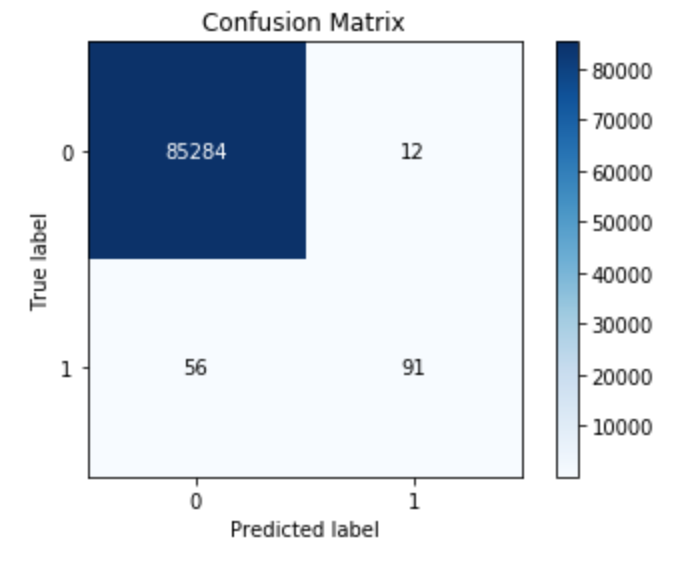
\includegraphics[scale=0.6]{cm-example}
\caption{Example Confusion Matrix plot.}
\label{fig:cm-example}
\end{figure}

From these, precision, recall and F measure scores can therefore be calculated and a classification report summary can be shown. 

\subsection{Visual Inspections}

\textbf{Precision-Recall Curves and ROC}\\
When classifying, the true positive rate (TPR) and false positive rate (FPR) changes for increasing values of precision and recall. This can be visualised by looking at TPR-FPR curves. This gives an indication of how the trade-off varies for differing values.

Taking the area under this curve is known as AUC, therefore gives an overall statistic for comparing classifiers. 

\textbf{GAN loss function graphs and generated data visualising}\\
With GANs, the way in which we can visualise performance is different to others due to it's specific adversarial nature. Two prominent use cases for GANs is to view the loss function graph for the generator and discriminator networks to see how the two networks fight with each other. In an ideal, theoretical world, we would expect to see the two loss curves converging to some stable value, which indicates the two networks can no longer improve or better themselves. 

Also, seeing as a large part of the GAN architecture is generating data, we can inspect this to see if it looks appropriate. A common example with the MNIST dataset is to see if the generated images look like handwritten digits. In this case, we can inspect the shape and distribution of the generated fraud transactions and view them side-by-side with real fraud transactions to see if any similarities have been picked up by the network.

\section{Results Overview}
\subsection{Baseline Models}
\subsubsection{Results Table}

Here, I simply report the table of results (see table~\ref{table:baseline-results} below) for the baseline classifiers, for every type of resampling method. These results came from the cross-validation described in the previous two chapters.

\begin{table}[H]  
  \centering
  \begin{tabular}{ccccc}
    \toprule
     Classifier & F1 & Precision & Recall & AUC-ROC \\ \midrule
     \textbf{Original Dataset} \\ \midrule
    LogisticRegression & 0.679526 &  0.858680 & 0.585366 & 0.792588 \\
    KNeighborsClassifier & 0.777306 &  0.834855 & 0.739837 & 0.869780\\
    LinearSVC  & 0.752517 &  0.887192  & 0.680894 & 0.840350 \\
    DecisionTreeClassifier & 0.648748 & 0.584061 & 0.747967 & 0.873483 \\
    RandomForestClassifier & 0.789572 &  0.867006  & 0.737805 & 0.868790\\
    MLPClassifier & 0.759672  & 0.801885 & 0.737805 & 0.868720 \\
    GaussianNB & 0.114077  & 0.061255 & 0.833333 & 0.905594 \\ \midrule
    \textbf{Under-Sampled Dataset} \\  \midrule
    
    LogisticRegression & 0.062811 &  0.032562 & 0.884146 & 0.919338 \\
    KNeighborsClassifier & 0.128275  & 0.069294 & 0.884146 & 0.931555\\
    LinearSVC  & 0.068514 &  0.035956 &  0.876016  & 0.912220 \\
    DecisionTreeClassifier & 0.026292 &  0.013374 & 0.892276 & 0.882144 \\
    RandomForestClassifier & 0.100256 &  0.053308 & 0.886179  & 0.928646\\
    MLPClassifier & 0.073166  & 0.038147 &  0.896341 & 0.928560 \\
    GaussianNB & 0.099017 &  0.052607 & 0.855691 & 0.914186 \\ \midrule
    
    \textbf{Over-Sampled Dataset} \\  \midrule
    
    LogisticRegression & 0.111965 &  0.059809 & 0.892276 & 0.933744 \\
    KNeighborsClassifier &0.625977  & 0.553314 & 0.786585 & 0.892538\\
    LinearSVC  & 0.118897  & 0.063827 & 0.871951  & 0.924837 \\
    DecisionTreeClassifier & 0.649036  & 0.661330 & 0.664634 & 0.831985 \\
    RandomForestClassifier &  0.801992 &  0.884864 & 0.745935  & 0.872869\\
    MLPClassifier & 0.673009  & 0.631834 & 0.752033 & 0.875552 \\
    GaussianNB & 0.100591  & 0.053461 & 0.855691 & 0.914668 \\ \midrule
    
    \textbf{SMOTE-Sampled Dataset} \\  \midrule
    
    LogisticRegression & 0.107417 &  0.057296 & 0.873984  & 0.924311 \\
    KNeighborsClassifier &0.481362  & 0.358277 & 0.829268 & 0.913002\\
    LinearSVC  & 0.118380 &  0.063560 & 0.865854  & 0.921825 \\
    DecisionTreeClassifier & 0.459940  & 0.336584 & 0.747967 & 0.872652 \\
    RandomForestClassifier &  0.805452  & 0.844639 & 0.782520 & 0.891119\\
    MLPClassifier & 0.678626 &  0.649623 & 0.731707 & 0.865467 \\
    GaussianNB & 0.107921 &  0.057627 & 0.855691 & 0.915657 \\
    
   \bottomrule
 \end{tabular}
 \caption{Baseline Models Results.}
\label{table:baseline-results}
\end{table}

\textbf{Key Observations}
\begin{enumerate}
\item \textbf{Original dataset results}: The results on the original dataset are fairly standard across the board, with certain classifiers achieving better F1 than others. Random Forest reports the best F1 score. 

\item \textbf{Under-Sampled dataset results}: When the data has been under-sampled, that is, a very large proportion of data has been taken away to balance the classes, we see that precision is dramatically affected. Hence, so are the F1 scores. This observation is perhaps somewhat intuitive given that if we think that we are removing information from the system, the model has less to learn on and hence more misclassifications of the genuine class will occur. 

\item \textbf{Over-Sampled dataset results}: Comparing this set of results with the original dataset, an observation can be made that on the whole, recall scores increase however precision scores suffer. Considering that this form of resampling is duplicating fraud data points, it is understandable why recall would increase. Here it is also observed that tree based classifiers remain high performers. 

\item \textbf{SMOTE dataset results}: Similarly the tree based classifiers perform better than the others. Some of the classifiers performed worse with SMOTE, which is perhaps due to how the model has learned differently from duplicated data vs different synthetic data. However, it is interesting to note that Random Forest and MLP remain consistent, which is a good sign as theoretically we would prefer to use SMOTE given that the data points are different. 
 
\end{enumerate}

\subsubsection{Further Tuning the RandomForest }
Seeing as Random Forest was clearly a classifier that performed well across the board with this type of application/data, I took some of it's most prominent parameters and performed a grid search, to see how much of an improvement I could get from further tuning. The tuning was done on the SMOTE data, this was because it gave interesting improvements on recall on the dataset, compared with that of the original dataset. This is interesting because for other classifiers, performing something like smote dramatically kills precision. 

The parameters I searched across were: \\
\begin{enumerate}
\item \textbf{n\_estimators=\{10, 100, 200\}}
\item \textbf{criterion=\{'gini', 'entropy'\}}
\item \textbf{max\_features=\{'auto', 'log2'\}}
\end{enumerate}

The original F1, precision and recall respectively were: \textbf{0.805452   0.844639  0.782520}.\\
The best parameters, found by searching were:\\
\textbf{criterion='entropy', max\_features='auto', n\_estimators=200.}\\

Table~\ref{table:rf-tuning} below shows the results of this tuning.


\begin{table}[H]  
  \centering
  \begin{tabular}{cccc}
    \toprule
           		& F1 & Precision & Recall \\ \midrule
    Before Tuning & 0.805452  & 0.844639  & 0.782520  \\
    After Tuning & 0.827025 & 0.853782 & 0.813008  \\
   \bottomrule
 \end{tabular}
 \caption{Random Forest Parameter Tuning Results.}
\label{table:rf-tuning}
\end{table}


\subsection{CNN Models}

\subsubsection{CNN Version 1 Results}

Below, I summarise the results of the version 1 models. Table~\ref{table:cnnv1-results-original} shows the results based on using the original dataset and Table~\ref{table:cnnv1-results-smote} shows those using SMOTE as a dataset resampling technique inside the cross-validation.

\begin{table}[H]  
  \centering
  \begin{tabular}{ccccc}
    \toprule
           		& F1 & Precision & Recall & AUC-ROC \\ \midrule
    CNN Model 1 & 0.809863 & 0.881838 & 0.760163 & 0.879979  \\
    CNN Model 1.2 & 0.821249 & 0.881579 & 0.774390 & 0.887097  \\
   \bottomrule
 \end{tabular}
 \caption{CNN Model 1 Results for Original Dataset.}
\label{table:cnnv1-results-original}
\end{table}

%\begin{table}[H]  
%  \centering
%  \begin{tabular}{ccccc}
%    \toprule
%           		& F1 & Precision & Recall & AUC-ROC\\ \midrule
%    CNN Model 1 & 0.815548 & 0.898798 & 0.760163  \\
%    CNN Model 1.2 &  0.826265 & 0.890820 & 0.778455 \\
%   \bottomrule
% \end{tabular}
% \caption{CNN Model 1 Results for Original Dataset (with lower learning rate).}
%\label{table:cnnv1-results-original-lowlr}
%\end{table}
%
%0.901706  0.645623   0.586726  0.804878 00:02:48.493895
%CNN Model 1.2  0.906084  0.596756   0.552336  0.815041

\begin{table}[H]  
  \centering
  \begin{tabular}{ccccc}
    \toprule
           		& F1 & Precision & Recall & AUC-ROC\\ \midrule
    CNN Model 1 & 0.645623 &  0.586726 & 0.804878 & 0.901706 \\
    CNN Model 1.2 &  0.596756  & 0.552336 & 0.815041 & 0.906084\\
   \bottomrule
 \end{tabular}
 \caption{CNN Model 1 Results for SMOTE Dataset.}
\label{table:cnnv1-results-smote}
\end{table}

Key observations from these results are that the original dataset performs better, without any resampling involved and that the learning rate parameter of the Adam optimiser plays a key role in the model tuning. In the case of the original dataset results, a learning rate that is a factor of 10 lower than the default value ($lr = 0.00001$) leads to better scores. In the case of the SMOTE data, a higher learning rate was better. 

%\begin{table}[H]  
%  \centering
%  \begin{tabular}{cccc}
%    \toprule
%           		& F1 & Precision & Recall \\ \midrule
%    CNN Model 1 & 0.522428  & 0.479291 & 0.762195  \\
%    CNN Model 1.2 &  0.594949  & 0.525301 & 0.815041 \\
%   \bottomrule
% \end{tabular}
% \caption{CNN Model 1 Results for SMOTE Dataset (with lower learning rate).}
%\label{table:cnnv1-results-smote-lowlr}
%\end{table}

\subsubsection{CNN Version 2 Results}

Below, I report the best results for the version 2 model. Table~\ref{table:cnnv2-results-original} shows the results for the default case of the model. This default case uses 100 as the batch-size and 5 for the window-height. These correspond to how many transactions are taken and temporally ordered and the height of the sliding window, respectively. 

\begin{table}[H]  
  \centering
  \begin{tabular}{ccccc}
    \toprule
           		& F1 & Precision & Recall & AUC-ROC \\ \midrule
    CNN Model 2 & 0.674887 & 0.934534 & 0.530247 & 0.952731  \\
 
   \bottomrule
 \end{tabular}
 \caption{CNN Model 2 Results for batch-size = 100, window-height = 5.}
\label{table:cnnv2-results-original}
\end{table}

Having a recall of $ \approx0.53 $ is not particularly great for the problem at hand, despite the impressive precision of the model. Therefore I do a search across some varying parameter values, to give an indication of the improvements to the results that can be made. Table~\ref{table:cnnv2-results-tuning} reports the results of tuning these two parameters.

\begin{table}[H]  
  \centering
  \begin{tabular}{ccccc}
    \toprule
     (batch-size , window-height) & F1 & Precision & Recall & AUC-ROC \\ \midrule
    (100 , 5) & 0.674887 & 0.934534 & 0.530247 & 0.952731  \\
    (200 , 5) & 0.683986 & 0.966952 & 0.531695 & 0.938287 \\
    (500 , 5) & 0.607998 &1.0 & 0.439607 & 0.924830 \\
    (100 , 10) & 0.734242 & 0.933769 & 0.608294 & 0.930754 \\
    (200 , 10) & 0.715631 & 0.934084 & 0.586319 & 0.911789 \\
    (500 , 10) & 0.62118 & 0.962963 & 0.459854 & 0.902490\\
   \bottomrule
 \end{tabular}
 \caption{CNN Model 2 Results for Varying (batch-size , window-height) Values.}
\label{table:cnnv2-results-tuning}
\end{table}

These results indicate that perhaps a smaller batch size but higher window height performs the best. 

\subsection{GAN Models}
In this section I report findings from the GAN approaches in application to the credit card fraud data. These results were all carried out on the original dataset . It is clear that this is a very experimental use-case with the low reported precision scores seen below, but the effects of network variations are still interesting nonetheless.

\subsubsection{GAN version 1 and it's variations}

In these versions, only the fraud data is being used, as the aim is to see how the GAN learns to model fraudulent transactions and to see what the loss curves look like. Below I describe the results from the variations on the adversarial training. 

\textbf{Version 1.1}

In this version, standard adversarial training is applied. Both the generator and discriminator are trained separately in each epoch.

Figure~\ref{fig:ganv1-losses} below shows the training losses for the model. It can be observed that between 500 and 1500 epochs, the generator improves and learns to fool the discriminator, but after this point the generator's loss slowly diverges as clearly the discriminator overpowers it, after eventually learning the data.

\begin{figure}[H]
\centering
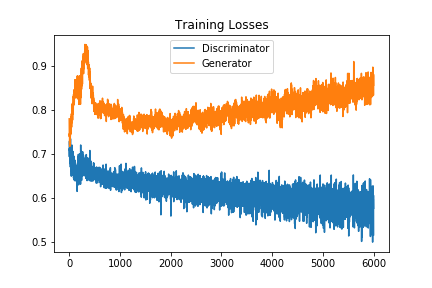
\includegraphics[scale=0.6]{GANv1-losses}
\caption{GANv1 Losses Graph.}
\label{fig:ganv1-losses}
\end{figure}

As an example of what generated output looks like and what was used to visualise fraud generation, Figure~\ref{fig:ganv1-generatedoutput} below shows the plot that was generated over 6 regular save intervals during training. In this particular case you can see the actual fraud data on the left and the generated fraud on the right, for every 1000 epochs. It can be observed that the model is slowly learning the shape and distribution of the data, albeit not perfectly. 

For the sake of brevity, I will omit future generated output plots for the following versions, but they can be seen in the Appendix. 

\begin{figure}[H]
\centering
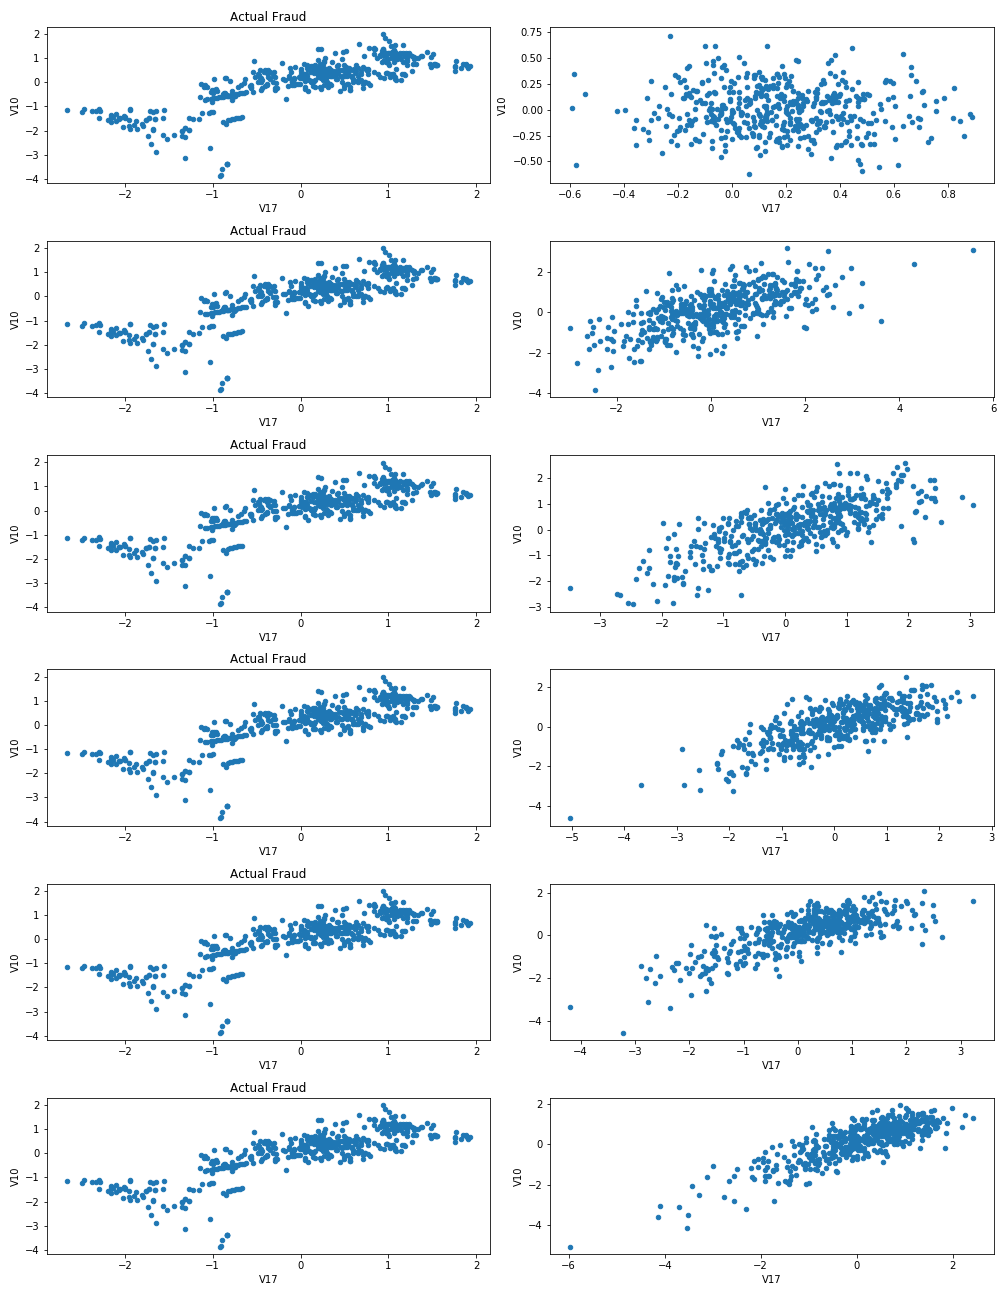
\includegraphics[scale=0.4]{GANv1-v17-v10-img_600}
\caption{GANv1 Generated Output Graph.}
\label{fig:ganv1-generatedoutput}
\end{figure}

\textbf{Version 1.2}

In version 1.2, I adapt the adversarial training to a setup whereby the discriminator is pre-trained alone for 500 epochs and then the generator is left to train for the rest. Figure~\ref{fig:ganv1.2-losses} shows the associated losses graph for this.

\begin{figure}[H]
\centering
\includegraphics[scale=0.6]{{{GANv1.2-losses}}}
\caption{GANv1.2 Losses Graph.}
\label{fig:ganv1.2-losses}
\end{figure}

The resulting graph for this variation is intuitive. After the discriminator is stopped training, the generator simply continues to learn to fool the now static discriminator. You can observe in the graph that the orange loss curve tends to zero very quickly afterwards. Figure~\ref{fig:GANv1.2-v17-v10-img_2} in the appendix shows that the generator concentrates a small subset that are able to fool the discriminator. 

\textbf{Version 1.3}

In version 1.3, the adversarial training was staggered between the two networks. Each network training separately for 500 epochs at a time. Figure~{fig:ganv1.3-losses} shows how the losses fluctuated in this scenario. Figure~\ref{fig:GANv1.3-v17-v10-img_2} in the appendix shows that the generator concentrates a small subset that are able to fool the discriminator. 

\begin{figure}[H]
\centering
\includegraphics[scale=0.6]{{{GANv1.3-losses}}}
\caption{GANv1.3 Losses Graph.}
\label{fig:ganv1.3-losses}
\end{figure} 

\textbf{Version 1.4}

In version 1.4, I used SMOTE data with standard adversarial training. Figure~{fig:ganv1.4-losses} shows how the losses fluctuated in this scenario. It is clear that  Figure~\ref{fig:GANv1.4-v17-v10-img_2} in the appendix shows how even with the increased size of the output data, the generator still focuses on a subset of the actual data distribution. 

\begin{figure}[H]
\centering
\includegraphics[scale=0.6]{{{GANv1.4-losses}}}
\caption{GANv1.4 Losses Graph.}
\label{fig:ganv1.4-losses}
\end{figure} 

\subsubsection{GAN version 2}

On the whole, the results for the second GAN model (using a previous CNN as a generator) showed relatively similar performance to the prior model, exhibiting similar loss and output graphs. It seems to be a common case with this data, that eventually the discriminator simply overpowers the generator in a slow diverging manner. Despite loading weights from the CNN model, the network continues quickly to expose any data distribution that it learns very quickly and after this point the loss just deteriorates as with previous models.

\subsubsection{Semi Supervised Results}
In this section I report findings from the semi-supervised approach to the GAN in application to the credit card fraud data. I report two main sets of results, one for a smaller amount of epochs and one for a larger amount, to give an indication of the differences in results and also because during experimentation these were key points.
Table~\ref{table:ganv1-ssl-original} below shows the reported scores for 600 epochs and 6000 epochs respectively. 

\textbf{Variation 1 - Using the original dataset in training (i.e the generator attempts to generate both fraud and non-fraud).}

\begin{table}[H]  
  \centering
  \begin{tabular}{ccccc}
    \toprule
           		& F1 & Precision & Recall & AUC-ROC \\ \midrule
    GANv1-SSL (600 epochs) & 0.00426  &  0.00213 & 0.93893  & 0.564891 \\
    GANv1-SSL (6000 epochs) & 0.01221   &   0.00615 & 0.83761 & 0.807437  \\
   
   \bottomrule
 \end{tabular}
 \caption{GANv1-SSL Results for Original Dataset.}
\label{table:ganv1-ssl-original}
\end{table}

It is clear from these results that the precision is very poor, despite rather good recall scores. An interesting thing to note from these is that increasing the amount of epochs that the network trains, decreases the recall but improves the precision. Although this improvement seems insignificant, this is just due to the amount of genuine examples compared with that of the true positives (the fraud). I report the confusion matrix for both cases below to show in terms of numbers, the improvement. Figure~\ref{fig:ganv1-ssl-cm-600} shows the confusion matrix for the 600 epochs run and you can see 57507 genuine transactions were misclassified as fraud. That is 81\% of all genuine transactions. In contrast, Figure~\ref{ig:ganv1-ssl-cm-6000} shows the confusion matrix for the 6000 epochs run and the false negative count has decreased to 22\%. In raw numbers, that is over 40,000 transactions that have been now correctly classified. So clearly, the increased epochs performs better and allows the network to learn better which transactions are genuine. 

\begin{figure}[H]
\centering
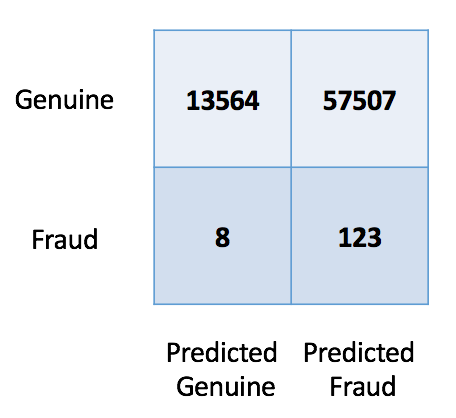
\includegraphics[scale=0.6]{ganv1-ssl-cm-600}
\caption{GANv1-SSL Confusion Matrix for 600 epochs.}
\label{fig:ganv1-ssl-cm-600}
\end{figure}

\begin{figure}[H]
\centering
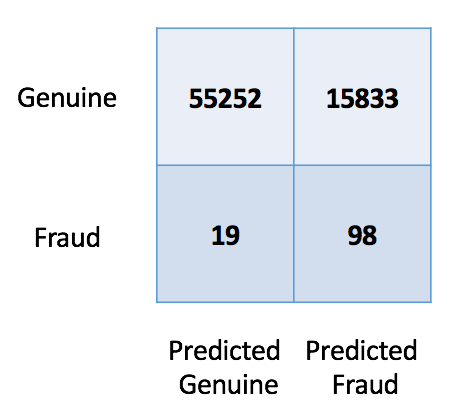
\includegraphics[scale=0.6]{ganv1-ssl-cm-6000}
\caption{GANv1-SSL Confusion Matrix for 6000 epochs.}
\label{fig:ganv1-ssl-cm-6000}
\end{figure}

Based on this observation it was fitting to try running with a number of epochs a factor of 10 above, to see if this improvement continues. 

\begin{table}[H]  
  \centering
  \begin{tabular}{ccccc}
    \toprule
           		& F1 & Precision & Recall & AUC-ROC \\ \midrule
    GANv1-SSL (30000 epochs) & 0.01365  &  0.00688 & 0.83871  & 0.813788 \\
    GANv1-SSL (60000 epochs) & 0.01410   &   0.00712 & 0.68293 & 0.759097  \\
   
   \bottomrule
 \end{tabular}
 \caption{GANv1-SSL increased epochs.}
\label{table:ganv1-ssl-original-2}
\end{table}

\textbf{Variation 2 - Similar to version 1, but ensuring the discriminator takes a 50:50 ratio of fraud and genuine transacations, from the real portion of the input.}

Here, when the discriminator takes a half batch of real and generated input, I ensure that the real input has an equal amount of fraud and genuine data. The results for this are as follows:

\begin{table}[H]  
  \centering
  \begin{tabular}{ccccc}
    \toprule
           		& F1 & Precision & Recall & AUC-ROC \\ \midrule
    GANv1-SSL (6000 epochs) & 0.00827  &  0.00415 & 0.98496  & 0.771414 \\
    GANv1-SSL (30000 epochs) & 0.71212  &  0.63514 & 0.81034  & 0.904792 \\
    GANv1-SSL (60000 epochs) & 0.00993   &   0.00499 & 0.85484 & 0.778857  \\
   
   \bottomrule
 \end{tabular}
 \caption{GANv1-SSL Variation 2 Results.}
\label{table:ganv1-ssl-halfhalf}
\end{table}

Table~\ref{table:ganv1-ssl-halfhalf} shows that there is a sweet spot at around 30000 epochs in which the classification portion of the GAN performs reasonably well in comparison to some of the results seen previously in the project. It also indicates how performance can fluctuate. 

\textbf{Variation 3 - Fraud data only, but classifying on both genuine and fraud.}
In this case, the network was not useful at all. Due to the fact that the network learns the shape of classification of fraud, it simply misclassified all benign transactions even for high epoch numbers. 


% Conclusion
\chapter{Conclusions}

The project was a success in that the work set out to be completed, was achieved, with extra work and experimentation than first anticipated. It was also an incredible learning process about the use of these types of models and how they behave.
To conclude, I will simply answer the primary question that the project started out with: \textbf{Can we apply these Deep Learning architectures to this problem?}. The answer, is yes we can apply them. The next thing would be to consider whether it was good or bad in applying them.

 I think it is clear that using convolutional based networks definitely has a place in the time-series and credit card fraud domain. This stems from both previous seen success, as mentioned with WaveNet and also from this project's experimentation with the CNN models applied to this data. With deep learning architectures like this, there are many variables and methods that can be undertaken to further tune and improve performance of the models. In this project, I scratched the surface of these but with further experimentation I suspect we could achieve even more comparable results. 

As for the GAN models, I do not think that applying these helps a great deal in the problem space. Although an interesting experiment, which showed that we can sample from the original dataset and train a model to learn what fraudulent transactions look like (with reasonable success), I suspect this would be limited when actually applying this to the real-world problem of credit card fraud detection. There is a obviously a fixed amount of information in a dataset and a theoretically optimal classifier would use all of that information. The GAN trained on the dataset does not actually create new information, it just tries to learn best the distribution of the original data. Therefore interesting hypothesises such as ''We use a GAN to generate new fraud with which we can train other models with, to solve imbalance problems?'' appear to be negative. 
Using the GAN as a semi-supervised learning classifier was a very intriguing addition to the project and highlighted that in certain conditions, there was indication that this setup could work (in reference variation 2). However we have to also consider this in comparison to what we can already achieve with the 'simpler' baseline classifiers I started the project with. GANs would require a ton more data and would need to train for a very long time to uncover proportionally smaller incremental improvements. I therefore conclude that in this case it is perhaps better to expend effort tuning parameters and optimising something like the Random Forest Classifier, that we saw early on. 


%%%%%%%%%%%%%%%%%%%%%%%%%%%%%%%%%%%%%%%%%%%%%%%%%%%%%%%%%%%%%%%%%%%%%
% the bibliography
\newpage
\addcontentsline{toc}{chapter}{Bibliography}
\bibliographystyle{ieeetr}
\bibliography{references}

%%%%%%%%%%%%%%%%%%%%%%%%%%%%%%%%%%%%%%%%%%%%%%%%%%%%%%%%%%%%%%%%%%%%%

%%%%%%%%%%%%%%%%%%%%%%%%%%%%%%%%%%%%%%%%%%%%%%%%%%%%%%%%%%%%%%%%%%%%%
% the appendix

\appendix 

\chapter{GAN Generated Outputs}

\begin{figure}[H]
\centering
\includegraphics[scale=0.4]{{{GANv1.2-v17-v10-img_2}}}
\caption{GANv1.2 Generated Outputs for every 1000 epochs.}
\label{fig:GANv1.2-v17-v10-img_2}
\end{figure}

\begin{figure}[H]
\centering
\includegraphics[scale=0.4]{{{GANv1.3-v17-v10-img_2}}}
\caption{GANv1.3 Generated Outputs for every 1000 epochs.}
\label{fig:GANv1.3-v17-v10-img_2}
\end{figure}

\begin{figure}[H]
\centering
\includegraphics[scale=0.4]{{{GANv1.4-v17-v10-img_2}}}
\caption{GANv1.4 Generated Outputs for every 1000 epochs.}
\label{fig:GANv1.4-v17-v10-img_2}
\end{figure}

\chapter{Project Proposal}

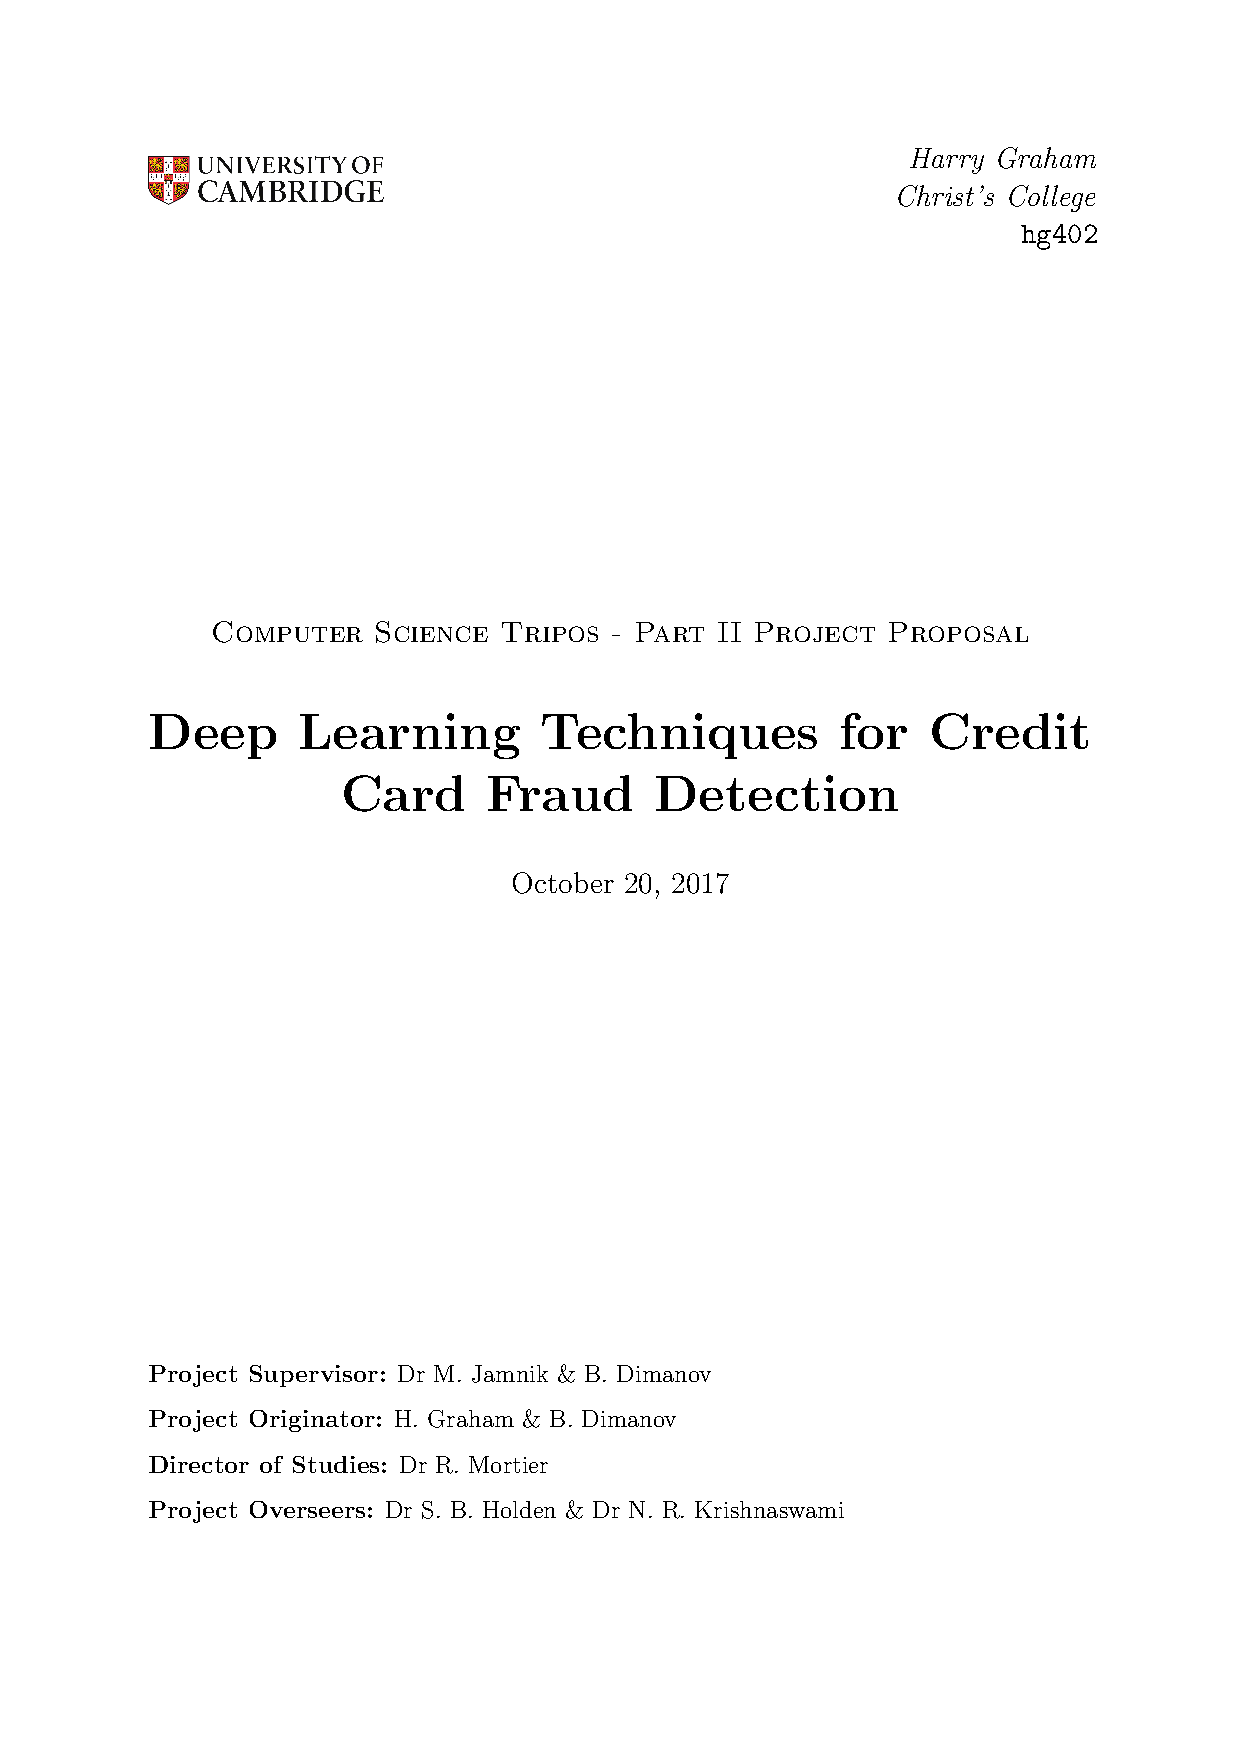
\includepdf[pages=-]{proposal.pdf}
%%%%%%%%%%%%%%%%%%%%%%%%%%%%%%%%%%%%%%%%%%%%%%%%%%%%%%%%%%%%%%%%%%%%%

\end{document}





